\newcommand{\PraxisTeam}{7391856}
\newcommand{\PraxisTitle}{A Hot Bath: Conserving Water Without Losing Uniformity}
% BEGIN PRAXIS MCM STYLE v4
% Praxis MCM house style v4. Layout source; assemble with scripts.paper_template.
\documentclass[12pt,a4paper]{article}
\usepackage[left=1in,right=1in,top=0.95in,bottom=0.8in,headheight=15pt]{geometry}
\usepackage{amsmath,amssymb,amsthm}
\usepackage{newtxtext,newtxmath}
\usepackage{booktabs,array,graphicx,xcolor,caption,float,etoolbox,fvextra,fancyhdr,lastpage,titlesec,titletoc,needspace,indentfirst}
\usepackage[hidelinks,pdfauthor={},pdftitle={\PraxisTitle}]{hyperref}
\urlstyle{same}\Urlmuskip=0mu plus 1mu
\usepackage{pgfplots}
\pgfplotsset{compat=1.17}
\usepgfplotslibrary{fillbetween,groupplots}
\usetikzlibrary{arrows.meta,positioning,calc}
\definecolor{main}{HTML}{0072B2}
\definecolor{accent}{HTML}{D55E00}
\definecolor{muted}{HTML}{7A7F85}
\definecolor{light}{HTML}{B8BDC2}
\definecolor{oigreen}{HTML}{009E73}
\definecolor{oiorange}{HTML}{E69F00}
\definecolor{oisky}{HTML}{56B4E9}
\definecolor{oiyellow}{HTML}{F0E442}
\definecolor{teal}{HTML}{17766E}
\definecolor{clay}{HTML}{9E6440}
\definecolor{slate}{HTML}{5D696E}
\definecolor{sand}{HTML}{AAA69B}
% A4 is the project default; the applicable edition may also permit US Letter.
% Ordinary plot labels, ticks, legends and panel titles use the body size.
% A generator's local size options need an explicit matching font profile;
% imported standalone figures also require final-size PDF inspection.
\pgfplotsset{tick label style={font=\normalsize},label style={font=\normalsize},legend style={font=\normalsize},title style={font=\normalsize}}
\linespread{1.12}
\setlength{\parindent}{2em}\setlength{\parskip}{3pt}
\titleformat{\section}{\Large\bfseries}{\thesection}{0.6em}{}
\titleformat{\subsection}{\large\bfseries}{\thesubsection}{0.6em}{}
\titleformat{\subsubsection}{\normalsize\bfseries}{\thesubsubsection}{0.6em}{}
\titlespacing{\section}{0pt}{16pt plus 3pt}{8pt}
\titlespacing{\subsection}{0pt}{12pt plus 2pt}{6pt}
\titlespacing{\subsubsection}{0pt}{10pt plus 2pt}{5pt}
\setcounter{secnumdepth}{3}
% A dedicated summary heading restores ordinary paragraph indentation after
% the centered heading; other centered content, lists and captions keep their roles.
\makeatletter
\newcommand{\PraxisSummaryHeading}[1]{\begin{center}{\Large\bfseries #1}\end{center}\@afterindenttrue\@afterheading}
\makeatother
\captionsetup{font=normalsize,labelfont=bf,labelsep=period,justification=centering}
\captionsetup[table]{position=above,skip=5pt}\captionsetup[figure]{position=below,skip=7pt}
\setcounter{tocdepth}{2}
\setlength{\emergencystretch}{3em}
\pagestyle{fancy}\fancyhf{}
\fancyhead[L]{Team \# \PraxisTeam}\fancyhead[R]{Page \thepage{} of \pageref{LastPage}}
\renewcommand{\headrulewidth}{0.4pt}
\makeatletter\setlength{\@fptop}{0pt}\setlength{\@fpsep}{14pt}\setlength{\@fpbot}{0pt plus 1fil}\makeatother
\AtBeginEnvironment{thebibliography}{\normalsize}
% Two TOC levels by default; a shared component can select three when useful.
\titlecontents{section}[1.8em]{\addvspace{5pt}\bfseries}{\contentslabel{1.8em}}{}{\titlerule*[.6pc]{.}\contentspage}
\titlecontents{subsection}[4.1em]{}{\contentslabel{2.3em}}{}{\titlerule*[.6pc]{.}\contentspage}
\titlecontents{subsubsection}[7.3em]{}{\contentslabel{3.2em}}{}{\titlerule*[.6pc]{.}\contentspage}
% END PRAXIS MCM STYLE
\usepackage{placeins}
\begin{document}
\thispagestyle{empty}\begin{center}\begin{tabular*}{\linewidth}{@{\extracolsep{\fill}}ccc}
\parbox[t]{.30\linewidth}{\centering\textbf{Problem Chosen}\\[5pt]{\fontsize{26}{30}\selectfont\bfseries A}}&
\parbox[t]{.30\linewidth}{\centering\textbf{2016\\MCM/ICM\\Summary Sheet}}&
\parbox[t]{.30\linewidth}{\centering\textbf{Team Control Number}\\[5pt]{\fontsize{26}{30}\selectfont\bfseries\PraxisTeam}}
\end{tabular*}\end{center}\vspace{-4pt}\hrule\vspace{10pt}
\begin{center}{\LARGE\bfseries A Hot Bath: Conserving Water Without Losing Uniformity}\end{center}
\PraxisSummaryHeading{Summary}
Conserving bath water requires two decisions: when to replace lost heat, and whether that heat can reach the coldest region in time. Our strategy replenishes before a remote cold region loses its reserve and permits waiting only while a feasible continuation remains; a temperature allowance is not a faucet-start trigger.

We prove coast-then-hold optimal for a perfectly mixed bath. A conservative three-dimensional thermal network then resolves the temperature differences hidden by that benchmark. Coefficients have correlation-based anchors and explicit scenario ranges. Comfort is represented by a floor in every cell and ceiling/spread limits outside a 0.15 m inlet zone; this does not resolve jet or skin-film safety.

For 164.25 L initially at 40°C, a 30-minute bath with a 39°C floor needs \textbf{24.14 L} under the best accepted constant trickle, started at minute zero. The buffered six-stage policy waits five minutes, replenishes for fifteen and coasts for ten, using \textbf{21.48 L} (11\% less). Independent continuous-time checks qualify it on three networks. The mixed optimum is 16.01 L and the spatial energy lower bound 15.41 L; the searched spatial policy is not a global optimum.

Transport changes the value of waiting. A local sensitivity criterion compares the extra rate needed after a delay with the water saved while the faucet is off. Stronger mixing permits a qualified 780 s wait followed by a pulse; at least 790 s is impossible for any allowed common inflow on that fixed network. Weak mixing has a separate all-control obstruction. An axial model reproduces the timing change, while cooler-than-mean overflow rules out excess outlet heat loss as its explanation in the tested baselines.

At equal volume, a deep-narrow tub needs 17.48 L; greater body displacement/contact raises demand to 28.11 L. Stronger modeled mixing lowers constant-flow demand from 24.14 to 19.40 L, but added surface loss raises it to 23.04 L; assumed foam lowers it to 10.37 L. The closed-network mixing times are 1012/304/101 s across the tested diffusivities. Both synthetic two-probe trials retain all seven prior mixing values: measured contrasts do not uniquely identify motion or certify a waiting time. The controller instead waits or reduces inflow only while every compatible model has a checked continuation; inconsistent readings require reassessment. These are conditional model results. The one-page guide explains the resulting actions.

\textbf{Keywords:} thermal network; energy balance; lower bound; optimal control; sensitivity analysis

\clearpage\tableofcontents\clearpage
\clearpage
\section{Problem formulation}
The task is to preserve both warmth and spatial uniformity in an overflowing, unheated tub, and to examine geometry, the bather and motion, and a bubble-bath layer [1]. The report separates physical requirements from preference assumptions. There is no supplied temperature record or measured heat-transfer coefficient to fit.

The decisions are a bounded inlet-flow history and its starting time; constant trickles, six-stage schedules and observation-updated actions are distinguished. The tub is already full: added water displaces an equal volume through the overflow. The horizon is 1,800 s. Our baseline requires every cell average to stay at or above 39°C, and requires the cell averages outside a 0.15 m jet-mixing zone around the inlet to stay at or below 41°C and within an instantaneous spread of 1.5°C. These choices operationalize comfort; they are not medical limits or numbers specified by the problem, and the jet zone is an assumption justified in Section 2.

\begin{equation}J=1000\int_0^{t_f}q(t)\,dt\end{equation}
\begin{equation}T_i(t)\geq T_{\min}\ \ (\forall i),\qquad T_i(t)\leq T_{\max},\quad \max_{i\in\Omega}T_i(t)-\min_{i\in\Omega}T_i(t)\leq\Delta\ \ (i\in\Omega)\end{equation}
Here $\Omega$ is the set of cells outside the inlet jet zone, $q$ is in m³/s and J is in litres. We prioritize the least water within the constraints, rather than assigning arbitrary weights to unlike units. Tightening the temperature tolerance is a separate scenario. Zero flow is admitted: if the initial stored heat suffices, using no added water is globally water-minimal.

\begin{table}[ht]\centering\normalsize\caption{Where each requirement is answered}\label{tab:1}
\begin{tabular}{@{}>{\raggedright\arraybackslash}p{0.4487\dimexpr\linewidth-2\tabcolsep\relax}>{\raggedright\arraybackslash}p{0.5513\dimexpr\linewidth-2\tabcolsep\relax}@{}}
\toprule
Requirement & Where answered \\ \midrule
Temperature in space and time & Sections 3, 5–7; Figures \ref{fig:spatial}–\ref{fig:temperature} \\
Water-use strategy and its scope & Sections 4, 6–7 and 12 \\
Tub/body geometry, size and temperature & Section 8 \\
Motion and bubble-bath additive & Section 9 \\
Validation and sensitivity & Sections 8–11 \\
One-page non-technical explanation & Section 13 \\ \bottomrule
\end{tabular}
\end{table}
Table \ref{tab:1} locates each answer. Spatial temperature means a control-volume average. It does not bound the unresolved temperature of a faucet jet or a skin-contact film. This distinction determines which practical conclusions the simulation can support.

\textbf{Modeling options.} The lumped model supplies a proved benchmark; the conservative network resolves cold regions with an explicit mixing parameter [5]. A velocity solver needs jet and turbulence data unavailable here. Table \ref{tab:2} compares their roles.

\begin{table}[ht]\centering\normalsize\caption{Modeling options compared}\label{tab:2}
\begin{tabular}{@{}>{\raggedright\arraybackslash}p{0.2137\dimexpr\linewidth-6\tabcolsep\relax}>{\raggedright\arraybackslash}p{0.2564\dimexpr\linewidth-6\tabcolsep\relax}>{\raggedright\arraybackslash}p{0.2778\dimexpr\linewidth-6\tabcolsep\relax}>{\raggedright\arraybackslash}p{0.2521\dimexpr\linewidth-6\tabcolsep\relax}@{}}
\toprule
Option & Resolves & Evidence it needs & Role here \\ \midrule
Lumped (Newton) & Mean temperature & Two loss coefficients & Proved benchmark \\
Thermal network & Cells, heat paths, overflow & Loss, body and mixing coefficients & Decision model \\
Flow solver & Velocity and buoyancy & Turbulence closure, jet data & Not used \\ \bottomrule
\end{tabular}
\end{table}
\section{Assumptions and parameterization}
The problem supplies no calibrated coefficients. Table \ref{tab:3} separates baseline inputs by status; scenarios test the important assumptions.

\begin{table}[ht]\centering\normalsize\caption{Baseline inputs}\label{tab:3}
\begin{tabular}{@{}>{\raggedright\arraybackslash}p{0.3889\dimexpr\linewidth-4\tabcolsep\relax}>{\raggedright\arraybackslash}p{0.4017\dimexpr\linewidth-4\tabcolsep\relax}>{\raggedright\arraybackslash}p{0.2094\dimexpr\linewidth-4\tabcolsep\relax}@{}}
\toprule
Quantity & Baseline / units & Status \\ \midrule
Tub L × W × H & 1.50 × 0.65 × 0.23 m & Assumed geometry \\
Displaced body volume / area & 0.060 m³ / 1.15 m² & Assumed \\
Water density / heat capacity & 1000 kg/m³ / 4180 J/(kg K) & Rounded constants \\
Air / skin / inlet temperature & 22 / 34 / 50°C & Fixed reservoirs \\
Surface / wall / body coefficient & 25 / 6.5 / 25 W/(m² K) & Correlation-based (next page) \\
Mixing diffusivity $D$ & 0.001 m²/s & Uncalibrated closure; range tested \\
Initial / lower / upper limit & 40 / 39 / 41°C & Preference scenario \\
Time / allowed spread & 1800 s / 1.5°C & Preference scenario \\ \bottomrule
\end{tabular}
\end{table}
\textbf{A1. Constant density and heat capacity.} Water properties change by under 1\% between 39 and 41°C, and the constants are rounded values, not an evaluated IAPWS table [3]. \emph{Reason:} the resulting capacity error is small next to the loss coefficients.

\textbf{A2. Linear exchange.} Newton’s law [2] approximates the narrow temperature span. Surface loss includes convection, radiation and evaporation once; evaporative volume change is neglected. Room-temperature linearization understates near-40°C sensitivity by about 7\% of total loss in an independent estimate, within the tested coefficient range.

\textbf{A3. Skin held at a fixed temperature.} \emph{Reason:} thermoregulation is outside the problem; skin temperature is varied (32 and 36°C) instead of resolved.

\textbf{A4. Prescribed surface stream.} Water traverses the top row nearest the centre line (half a cell off it for even row counts). Alternative paths and whole-section flow are tested in Section 11; the route is assumed, not measured.

\textbf{A5. Mixing as one effective diffusivity $D$.} Motion is represented by $D$, with a separate surface-loss scenario. \emph{Reason:} molecular diffusion alone would not represent circulation; $D$ is anchored only by an order-of-magnitude scaling (Section 2) and is tested over a range; vertical mixing is tested separately in Section 9.

\textbf{Parameter provenance.}

No temperature record exists to fit, so each coefficient is derived from a textbook relation or tied to a published measurement where one exists, and given a range; where nothing exists (mixing, the exposed fraction, the air and skin temperatures) the value is an assumption and is labelled as one. Surface loss sums natural convection above a hot horizontal surface ($\mathrm{Nu}=0.15\,\mathrm{Ra}^{1/3}$ for $10^{7}<\mathrm{Ra}<10^{11}$, length $A/P$ [5]; here $\mathrm{Ra}=1.9\times10^{7}$), linearized radiation (emissivity 0.96) and evaporation by the Lewis analogy. For open water at 40°C in 22°C air at 50\% humidity the parts are 4.7, 6.1 and 24.6 W/(m² K) (0.66 kg/m² h evaporated), 35.4 in total. A bather covers part of the surface; with an assumed exposed fraction of 0.7 the central value is 24.8, and we use 25 within the range 17–37, which spans exposed fractions of 0.5 to 1.0. Evaporation correlations differ by tens of percent, so this is a scenario range, not a measured one.

A 5 mm shell (0.19 W/(m K)), with inside/outside films 300/8 W/(m² K), gives a series coefficient 6.5, with range 4.7–8.4; these are typical inputs. Menzies et al. observed rectal rise 0.9 ± 0.3°C after 30 min shoulder-depth immersion at 40°C [6]. For mass 73 kg and heat capacity 3470 J/(kg K), an assumed mean rise 1–2°C implies uptake 141–281 W and equivalent exchange 20–41 W/(m² K) at fixed 34°C skin. We use 25. Mean rise and driving difference are assumptions: this is a scale anchor, not calibration. Body capacity is about 37\% of water capacity; its delayed warming is tested in Section 11.1.

The assumed scaling $D\approx0.1u'\ell$ gives $1\times10^{-4}$/$1\times10^{-3}$/$6\times10^{-3}$ m²/s for velocity/eddy-length pairs (0.02 m/s, 0.05 m), (0.1, 0.1) and (0.3, 0.2). We use 0.001 and test 0.0003–0.003; these are circulation scenarios, not measured diffusivities.

Table \ref{tab:4} summarizes the coefficient anchors and ranges. The 39–41°C window is a preference, not a safety standard [6]. Inlet-cell maxima increase 40.55/40.76/41.00°C on the three meshes: the point source heats less water per cell. Ceiling/spread therefore exclude a 0.15 m inlet zone, assuming no bather occupies the jet; the floor covers every cell, as required by Section 4. Section 11 checks constrained quantities.

\begin{table}[ht]\centering\normalsize\caption{Coefficient anchors and the values used}\label{tab:4}
\begin{tabular}{@{}>{\raggedright\arraybackslash}p{0.2051\dimexpr\linewidth-6\tabcolsep\relax}>{\raggedright\arraybackslash}p{0.3462\dimexpr\linewidth-6\tabcolsep\relax}>{\raggedright\arraybackslash}p{0.2350\dimexpr\linewidth-6\tabcolsep\relax}>{\raggedright\arraybackslash}p{0.2137\dimexpr\linewidth-6\tabcolsep\relax}@{}}
\toprule
Coefficient & Relation or anchor & Derived value & Used (range tested) \\ \midrule
Surface, W/(m² K) & Convection + radiation + evaporation [5] & 35.4 open; 24.8 at 70\% & 25 (17–37) \\
Shell, W/(m² K) & Series resistance, typical shell values & 6.5 (4.7–8.4) & 6.5 (4.5–8.5) \\
Body, W/(m² K) & Uptake implied by core rise [6] & 20–41 at fixed skin & 25 (12–40) \\
Mixing $D$, m²/s & Mixing-length scaling & $1\times10^{-4}$ to $6\times10^{-3}$ & 0.001 (0.0003–0.003) \\ \bottomrule
\end{tabular}
\end{table}
\section{Well-mixed thermal model}
\begin{table}[ht]\centering\normalsize\caption{Symbols}\label{tab:5}
\begin{tabular}{@{}>{\raggedright\arraybackslash}p{0.2350\dimexpr\linewidth-2\tabcolsep\relax}>{\raggedright\arraybackslash}p{0.7650\dimexpr\linewidth-2\tabcolsep\relax}@{}}
\toprule
Symbol & Meaning \\ \midrule
C & Heat capacity of the water, J/K \\
$H_a$, $H_b$ & Air/shell and body conductance, W/K \\
$T_a$, $T_b$, $T_{\mathrm{in}}$ & Room, skin and inlet temperature, °C \\
$T_{\min}$, $T_{\max}$ & Lower and upper limit, °C \\
$q$, J & Inlet flow, m³/s; added water, L \\
$D$ & Effective mixing diffusivity, m²/s \\ \bottomrule
\end{tabular}
\end{table}
Using the notation in Table \ref{tab:5}, let $C$ be total water heat capacity, $H_a$ the air/shell conductance and $H_b$ the body conductance. A well-mixed overflow has the same temperature as the bath. Integrating the physical energy balance gives

\begin{equation}C\dot T=H_a(T_a-T)+H_b(T_b-T)+\rho c_pq(T_{\mathrm in}-T)\end{equation}
\begin{equation}C=\rho c_p(LWH-V_b),\quad H_b=h_bA_b\end{equation}
\begin{equation}H_a=h_s fLW+h_w\{LW+2H(L+W)\}\end{equation}
The foam multiplier $f$ equals one without a layer. Setting $q=0$, define $H=H_a+H_b$ and $T_e=(H_aT_a+H_bT_b)/H$. The cooling solution and first time to reach the lower limit are

\begin{equation}T(t)=T_e+(T_0-T_e)e^{-Ht/C}\end{equation}
\begin{equation}t_c=\frac{C}{H}\log\frac{T_0-T_e}{T_{\min}-T_e}\end{equation}
Baseline conductances are $H_a$ = 37.14 W/K and $H_b$ = 28.75 W/K, and C = 686,565 J/K. Thus $T_e$ = 27.24°C and $t_c$ = 14.17 min.

A heat-loss model must approach an environmental equilibrium rather than zero Celsius. This analytic boundary also supplies a direct check on signs and units. The benchmark describes mixing perfectly; the spatial model will test the cost of departing from that assumption.

\section{Mixed-model optimum and spatial energy bound}
Let $\ell(T)=H_a(T-T_a)+H_b(T-T_b)$ be the heat loss of the mixed bath, and let the inlet be hotter than every temperature considered. \textbf{Proposition 1.} Coasting to the lower limit and then holding it uses the least water, provided the holding rate is within the faucet bound. The proof has four steps.

\begin{proof}
\textbf{Step 1, an identity.} Dividing the balance by $T_{\mathrm{in}}-T$ and integrating over the horizon gives

\begin{equation}\int q\,dt=\frac{C}{\rho c_p}\log\frac{T_{\mathrm in}-T_0}{T_{\mathrm in}-T_f}+\int\frac{\ell(T)}{\rho c_p(T_{\mathrm in}-T)}\,dt\end{equation}
\textbf{Step 2, monotonicity.} The integrand $\ell(T)/(T_{\mathrm{in}}-T)$ has derivative $[H_a(T_{\mathrm{in}}-T_a)+H_b(T_{\mathrm{in}}-T_b)]/(T_{\mathrm{in}}-T)^2>0$, so it increases with $T$, and the logarithmic term increases with the final temperature. Water use is therefore an increasing functional of the temperature path.

\textbf{Step 3, the lowest admissible path.} Because $q\ge 0$, comparison with the no-flow solution gives $T(t)\ge T_c(t)$, the cooling curve of Section 3, and feasibility requires $T(t)\ge T_{\min}$. The pointwise lowest admissible path is $\max(T_c(t),T_{\min})$: coast until $T_c$ reaches $T_{\min}$, then hold.

\textbf{Step 4, attainability.} Holding $T=T_{\min}$ means $\dot T=0$, which needs the rate

\begin{equation}q_{\mathrm hold}=\frac{\ell(T_{\min})}{\rho c_p(T_{\mathrm in}-T_{\min})}\end{equation}
When this rate is within the bound, the path is feasible and, by Step 2, optimal.

\end{proof}
For the baseline, the mixed-model optimum adds 16.01 L: wait 14.17 min, then supply 1.012 L/min. Optimality is established for the mixed model; spatial policies are assessed separately.

\textbf{Proposition 2 (energy lower bound).} In the spatial model, suppose every cell satisfies $T_i(t)\ge T_{\min}$. Summing the cell balances gives $\sum_i C_iT_i(t_f)-CT_0=-\int L\,dt+\rho c_p\int q(T_{\mathrm{in}}-T_{\mathrm{out}})\,dt$, with $L$ the total loss. Each loss term increases with its cell temperature, and $H_a$ and $H_b$ are the sums of the cell conductances, so $L(t)\ge\ell(T_{\min})$. The outlet cell satisfies $T_{\mathrm{out}}\ge T_{\min}$, so $T_{\mathrm{in}}-T_{\mathrm{out}}\le T_{\mathrm{in}}-T_{\min}$, and the left side is at least $C(T_{\min}-T_0)$. Combining these three facts,

\begin{equation}J\geq\max\left(0,\frac{1000[\ell(T_{\min})t_f-C(T_0-T_{\min})]}{\rho c_p(T_{\mathrm in}-T_{\min})}\right)\end{equation}
The resulting 15.41 L is a genuine conditional lower bound, valid for any control, but it is not tight: the initial water is hotter than the floor and loses more heat, and limited mixing adds further cost. Section 7.1 shows how much of the gap an optimized schedule recovers.

\section{Spatial heat-network formulation}
The rectangular water envelope is divided into 8 × 4 × 3 cells. Each has a capacity $C_i$ and exchanges heat only across common faces. The cells whose centres lie within 0.15 m of the inlet cell form the jet zone (2, 9 and 22 cells on the 8 × 4 × 3, 12 × 6 × 4 and 16 × 8 × 6 meshes); $\Omega$ is the rest. Top cells lose heat to the room; bottom and side faces lose heat through the shell. The bather is represented by a smooth, three-dimensional displacement field and a distributed skin contact term.

\begin{equation}C_i\dot T_i=\sum_jg_{ij}(T_j-T_i)+H_{a,i}(T_a-T_i)+H_{b,i}(T_b-T_i)+S_i\end{equation}
\begin{equation}g_{ij}=\rho c_pD\frac{A_{ij}}{d_{ij}}\min(\phi_i,\phi_j),\quad C_i=\rho c_pV_i\end{equation}
Here $\phi$ is fluid fraction, $A_{ij}$ a face area and $d_{ij}$ the center separation. Symmetric $g_{ij}$ guarantees that internal heat exchange cancels when the equations are summed. $D$ is an effective mixing closure; molecular diffusion alone would not represent motion or buoyant circulation.

\begin{equation}w_i\propto\exp\left[-\frac{1}{2}\sum_{k=1}^3\left(\frac{x_{ik}-b_k}{s_k}\right)^2\right],\quad \sum_iw_i=1\end{equation}
\begin{equation}V_i=V_{\mathrm cell}-V_bw_i,\quad H_{b,i}=h_bA_bw_i\end{equation}
Baseline $\mathbf{b}=(0.55L,\,W/2,\,0.45H)$, with widths $\mathbf{s}=(0.40,0.16,0.12)$ m. Fluid fraction is $\phi_i=V_i/V_{\mathrm{cell}}$. The center $\mathbf{b}$ and widths $\mathbf{s}$ set the spatial distribution of body effects. Body volume and contact area remain independent inputs: shape is varied through $\mathbf{s}$ at fixed volume and area. This is a homogenized immersed-body representation, not an anatomically resolved obstruction. A cell whose occupied fraction reaches 0.95 is rejected rather than assigned a negative capacity.

A fixed envelope volume is preserved by balancing inlet and overflow. In the baseline the exact displaced-water volume is 164.25 L. Shape scenarios preserve envelope volume when isolating aspect-ratio effects. Volume scenarios deliberately change water depth and hence both storage and side-wall area.

\textbf{Spatial temperature distribution.}

Figure \ref{fig:spatial} locates cold regions across layers on one scale. The three layers share a color scale; distances are in metres.

\begin{figure}[ht]\centering
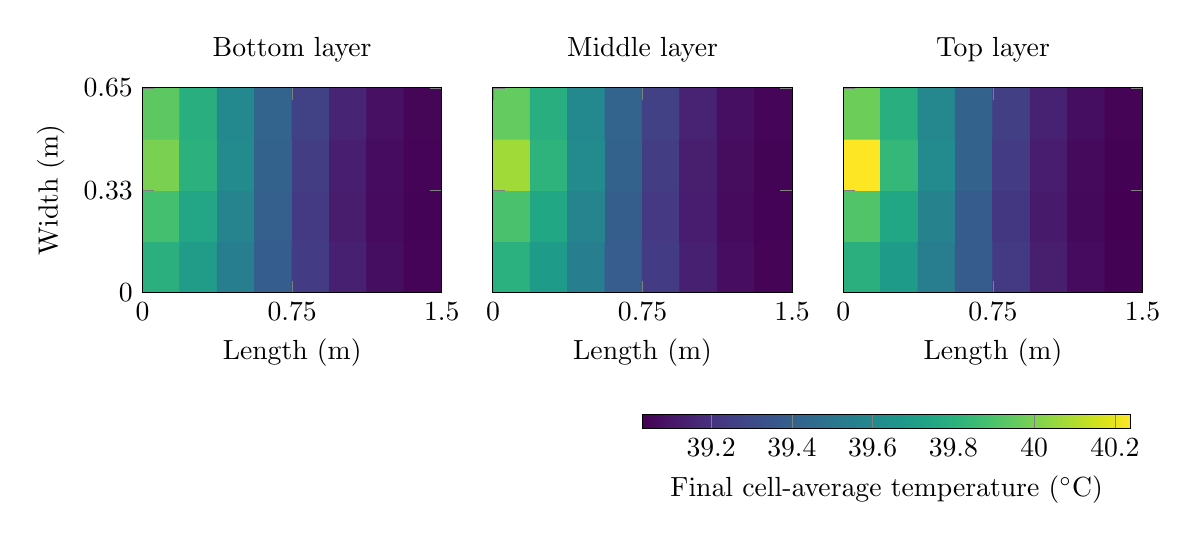
\begin{tikzpicture}
\begin{groupplot}[group style={group name=G,group size=3 by 1,horizontal sep=0.65cm,y descriptions at=edge left},width=3.8cm,height=2.6cm,scale only axis,enlargelimits=false,axis on top,xmin=0,xmax=1.5,ymin=0,ymax=0.65,colormap/viridis,point meta min=39.03,point meta max=40.2393,tick label style={font=\normalsize},label style={font=\normalsize},title style={font=\normalsize},xtick={0,0.75,1.5},ytick={0,0.325,0.65},xticklabel style={/pgf/number format/fixed}]
\nextgroupplot[title={Bottom layer},xlabel={Length (m)},ylabel={Width (m)}]
\addplot[matrix plot*,mesh/cols=8,point meta=explicit,shader=flat corner] table[meta expr=\thisrow{c}] {x y c
0.09375 0.08125 39.7942
0.28125 0.08125 39.6952
0.46875 0.08125 39.5455
0.65625 0.08125 39.3833
0.84375 0.08125 39.2419
1.03125 0.08125 39.1359
1.21875 0.08125 39.0704
1.40625 0.08125 39.0399

0.09375 0.24375 39.8787
0.28125 0.24375 39.7479
0.46875 0.24375 39.5754
0.65625 0.24375 39.3907
0.84375 0.24375 39.2339
1.03125 0.24375 39.1237
1.21875 0.24375 39.0629
1.40625 0.24375 39.037

0.09375 0.40625 39.9968
0.28125 0.40625 39.8029
0.46875 0.40625 39.6023
0.65625 0.40625 39.4065
0.84375 0.40625 39.2439
1.03125 0.40625 39.1297
1.21875 0.40625 39.0662
1.40625 0.40625 39.0391

0.09375 0.56875 39.9368
0.28125 0.56875 39.785
0.46875 0.56875 39.5983
0.65625 0.56875 39.4156
0.84375 0.56875 39.2619
1.03125 0.56875 39.1478
1.21875 0.56875 39.0772
1.40625 0.56875 39.0443
};
\nextgroupplot[title={Middle layer},xlabel={Length (m)}]
\addplot[matrix plot*,mesh/cols=8,point meta=explicit,shader=flat corner] table[meta expr=\thisrow{c}] {x y c
0.09375 0.08125 39.7955
0.28125 0.08125 39.6945
0.46875 0.08125 39.544
0.65625 0.08125 39.3815
0.84375 0.08125 39.24
1.03125 0.08125 39.1341
1.21875 0.08125 39.0688
1.40625 0.08125 39.0384

0.09375 0.24375 39.8925
0.28125 0.24375 39.7505
0.46875 0.24375 39.5747
0.65625 0.24375 39.3887
0.84375 0.24375 39.231
1.03125 0.24375 39.121
1.21875 0.24375 39.0608
1.40625 0.24375 39.0354

0.09375 0.40625 40.0681
0.28125 0.40625 39.8159
0.46875 0.40625 39.605
0.65625 0.40625 39.4073
0.84375 0.40625 39.2436
1.03125 0.40625 39.1286
1.21875 0.40625 39.0648
1.40625 0.40625 39.0377

0.09375 0.56875 39.9517
0.28125 0.56875 39.7878
0.46875 0.56875 39.5978
0.65625 0.56875 39.4143
0.84375 0.56875 39.2605
1.03125 0.56875 39.1463
1.21875 0.56875 39.0757
1.40625 0.56875 39.0429
};
\nextgroupplot[title={Top layer},xlabel={Length (m)}]
\addplot[matrix plot*,mesh/cols=8,point meta=explicit,shader=flat corner] table[meta expr=\thisrow{c}] {x y c
0.09375 0.08125 39.7937
0.28125 0.08125 39.6902
0.46875 0.08125 39.5386
0.65625 0.08125 39.3756
0.84375 0.08125 39.2339
1.03125 0.08125 39.1283
1.21875 0.08125 39.0635
1.40625 0.08125 39.0335

0.09375 0.24375 39.9087
0.28125 0.24375 39.7486
0.46875 0.24375 39.5675
0.65625 0.24375 39.38
0.84375 0.24375 39.2226
1.03125 0.24375 39.1139
1.21875 0.24375 39.0548
1.40625 0.24375 39.03

0.09375 0.40625 40.2393
0.28125 0.40625 39.8331
0.46875 0.40625 39.6048
0.65625 0.40625 39.4056
0.84375 0.40625 39.2416
1.03125 0.40625 39.1254
1.21875 0.40625 39.0604
1.40625 0.40625 39.0329

0.09375 0.56875 39.9695
0.28125 0.56875 39.7875
0.46875 0.56875 39.5933
0.65625 0.56875 39.409
0.84375 0.56875 39.2549
1.03125 0.56875 39.1408
1.21875 0.56875 39.0706
1.40625 0.56875 39.0381
};
\end{groupplot}
\begin{axis}[hide axis,scale only axis,width=0pt,height=0pt,at={(G c2r1.south)},anchor=north,yshift=-1.25cm,colormap/viridis,point meta min=39.03,point meta max=40.2393,colorbar horizontal,colorbar style={width=6.2cm,height=0.18cm,xlabel={Final cell-average temperature ($^\circ$C)},xlabel style={font=\normalsize},tick label style={font=\normalsize},xticklabel style={/pgf/number format/fixed,/pgf/number format/precision=1}}]
\addplot[draw=none] coordinates {(0,0)};
\end{axis}
\end{tikzpicture}
\caption{Final cell-average temperatures}\label{fig:spatial}
\end{figure}
The heat map and Figure \ref{fig:temperature} use the same archived trajectory. Exchange couples the horizontal layers into one three-dimensional network. The cold-region locations explain information lost by a mean or range; the mesh table tests resolution. These are homogenized cell averages, not resolved anatomy, recirculation or a faucet jet.

\section{Numerical solution and control search}
One surface stream carries the common $q$: hot water enters its first cell, upstream exchange transfers heat along the path, and its last cell overflows.

\begin{equation}S_1=\rho c_pq(T_{\mathrm in}-T_1),\quad S_i=\rho c_pq(T_{i-1}-T_i)\end{equation}
\begin{equation}\sum_i C_i\dot T_i=-\sum_iH_{a,i}(T_i-T_a)-\sum_iH_{b,i}(T_i-T_b)+\rho c_pq(T_{\mathrm in}-T_{\mathrm out})\end{equation}
This prescribed stream permits short circuit but does not establish excess outlet heat loss. Section 11.4 diagnoses its sign against a distinct whole-section closure; Section 11.1 changes the internal path at fixed inlet and overflow. Neither route is an inferred velocity field.

For a fixed flow, the network is affine linear. Augmenting the state by a constant one permits matrix-exponential propagation, avoiding a large forward-Euler step restriction [4]. A delayed-start policy has two exact constant-control segments.

\begin{equation}\dot{\mathbf{T}}=A(q)\mathbf{T}+\mathbf{b}(q),\quad \mathbf{z}(t+\tau)=e^{\widetilde{A}(q)\tau}\mathbf{z}(t)\end{equation}
Starts are tested at 0, 120, …, 1200 seconds. For each, rates from 0 to 3 L/min are bracketed on a 0.2 L/min grid; the first crossing of the lower-temperature requirement is refined by Brent’s root method. The search targets $T_{\min}+0.03$°C as numerical reserve, then checks the upper-temperature and spread limits at 5-second output intervals. Starts that already violate the floor are rejected.

This is a reproducible candidate search. Nonmonotone flow responses, untested delays, pulsed inputs, inlet relocation and feedback are not excluded by the calculation. A failed search means no candidate was accepted, not that every possible action is infeasible. The independent checks further examine the chosen trajectory between samples.

\section{Replenishment policies}
Figure \ref{fig:temperature} contrasts the mean, coldest cell and spatial range. Shading spans the coldest cell to the hottest cell outside the inlet jet zone.

\begin{figure}[ht]\centering
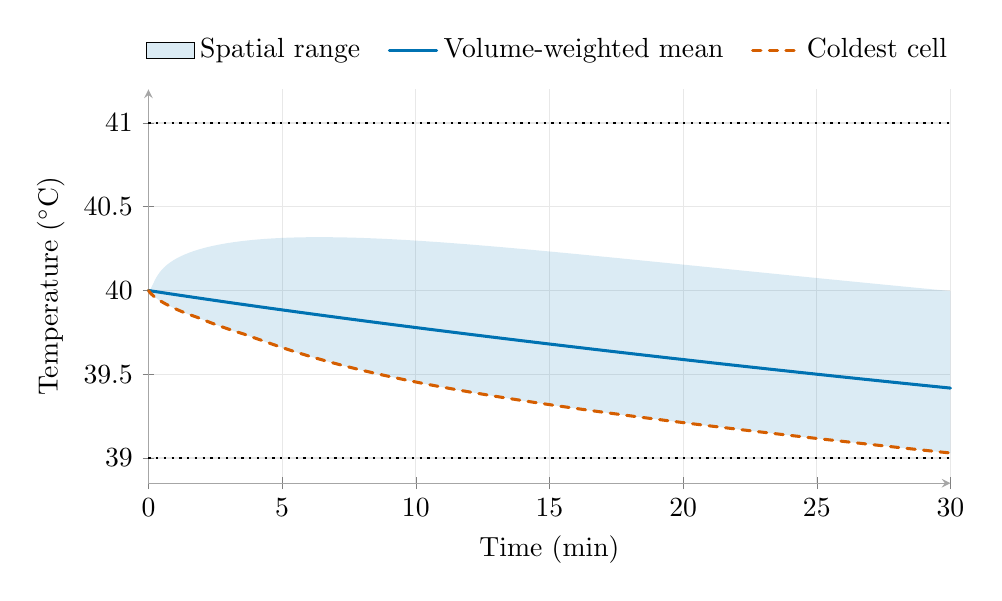
\begin{tikzpicture}
\begin{axis}[width=0.84\linewidth,
 height=5.0cm,
 scale only axis,
 xlabel={Time (min)},
 ylabel={Temperature ($^\circ$C)},
 axis lines=left,
 axis line style={gray!70},
 grid=major,
 grid style={gray!18},
 tick label style={font=\normalsize},
 label style={font=\normalsize},
 every axis plot/.append style={line cap=round},
 clip=false,
 xmin=0,
 xmax=30,
 ymin=38.85,
 ymax=41.2,
 legend style={font=\normalsize,draw=none,fill=none,at={(0.5,1.04)},anchor=south,legend columns=-1,/tikz/every even column/.append style={column sep=8pt},}]
\addplot[name path=lo1,draw=none,forget plot] coordinates {(0,40) (0.0833333,39.9833) (0.166667,39.9703) (0.25,39.9594) (0.333333,39.9498) (0.416667,39.941) (0.5,39.9329) (0.583333,39.9252) (0.666667,39.9179) (0.75,39.911) (0.833333,39.9043) (0.916667,39.8978) (1,39.8916) (1.08333,39.8856) (1.16667,39.8798) (1.25,39.8742) (1.33333,39.8688) (1.41667,39.8636) (1.5,39.8585) (1.58333,39.8536) (1.66667,39.8488) (1.75,39.8442) (1.83333,39.8395) (1.91667,39.834) (2,39.8285) (2.08333,39.8232) (2.16667,39.8179) (2.25,39.8128) (2.33333,39.8077) (2.41667,39.8026) (2.5,39.7977) (2.58333,39.7928) (2.66667,39.788) (2.75,39.7833) (2.83333,39.7786) (2.91667,39.774) (3,39.7695) (3.08333,39.765) (3.16667,39.7606) (3.25,39.7562) (3.33333,39.7519) (3.41667,39.7477) (3.5,39.7435) (3.58333,39.7394) (3.66667,39.7346) (3.75,39.7297) (3.83333,39.7249) (3.91667,39.7201) (4,39.7154) (4.08333,39.7108) (4.16667,39.7061) (4.25,39.7016) (4.33333,39.697) (4.41667,39.6921) (4.5,39.6874) (4.58333,39.6826) (4.66667,39.6779) (4.75,39.6733) (4.83333,39.6687) (4.91667,39.6642) (5,39.6597) (5.08333,39.6552) (5.16667,39.6508) (5.25,39.6464) (5.33333,39.6421) (5.41667,39.6378) (5.5,39.6336) (5.58333,39.6294) (5.66667,39.6253) (5.75,39.6211) (5.83333,39.6171) (5.91667,39.613) (6,39.609) (6.08333,39.6051) (6.16667,39.6012) (6.25,39.5973) (6.33333,39.5935) (6.41667,39.5897) (6.5,39.5859) (6.58333,39.5822) (6.66667,39.5785) (6.75,39.5748) (6.83333,39.5712) (6.91667,39.5676) (7,39.564) (7.08333,39.5605) (7.16667,39.557) (7.25,39.5536) (7.33333,39.5501) (7.41667,39.5467) (7.5,39.5434) (7.58333,39.54) (7.66667,39.5367) (7.75,39.5334) (7.83333,39.5302) (7.91667,39.5269) (8,39.5237) (8.08333,39.5205) (8.16667,39.5174) (8.25,39.5143) (8.33333,39.5112) (8.41667,39.5081) (8.5,39.5051) (8.58333,39.502) (8.66667,39.499) (8.75,39.4961) (8.83333,39.4931) (8.91667,39.4902) (9,39.4873) (9.08333,39.4844) (9.16667,39.4815) (9.25,39.4787) (9.33333,39.4759) (9.41667,39.4731) (9.5,39.4703) (9.58333,39.4675) (9.66667,39.4648) (9.75,39.462) (9.83333,39.4593) (9.91667,39.4567) (10,39.454) (10.0833,39.4513) (10.1667,39.4487) (10.25,39.4461) (10.3333,39.4435) (10.4167,39.4409) (10.5,39.4384) (10.5833,39.4358) (10.6667,39.4333) (10.75,39.4308) (10.8333,39.4283) (10.9167,39.4258) (11,39.4233) (11.0833,39.4209) (11.1667,39.4185) (11.25,39.416) (11.3333,39.4136) (11.4167,39.4112) (11.5,39.4088) (11.5833,39.4065) (11.6667,39.4041) (11.75,39.4018) (11.8333,39.3995) (11.9167,39.3971) (12,39.3948) (12.0833,39.3926) (12.1667,39.3903) (12.25,39.388) (12.3333,39.3858) (12.4167,39.3835) (12.5,39.3813) (12.5833,39.3791) (12.6667,39.3769) (12.75,39.3747) (12.8333,39.3725) (12.9167,39.3703) (13,39.3681) (13.0833,39.366) (13.1667,39.3638) (13.25,39.3617) (13.3333,39.3596) (13.4167,39.3574) (13.5,39.3553) (13.5833,39.3532) (13.6667,39.3512) (13.75,39.3491) (13.8333,39.347) (13.9167,39.3449) (14,39.3429) (14.0833,39.3408) (14.1667,39.3388) (14.25,39.3368) (14.3333,39.3348) (14.4167,39.3327) (14.5,39.3307) (14.5833,39.3287) (14.6667,39.3268) (14.75,39.3248) (14.8333,39.3228) (14.9167,39.3208) (15,39.3189) (15.0833,39.3169) (15.1667,39.315) (15.25,39.3131) (15.3333,39.3111) (15.4167,39.3092) (15.5,39.3073) (15.5833,39.3054) (15.6667,39.3035) (15.75,39.3016) (15.8333,39.2997) (15.9167,39.2978) (16,39.2959) (16.0833,39.294) (16.1667,39.2922) (16.25,39.2903) (16.3333,39.2885) (16.4167,39.2866) (16.5,39.2848) (16.5833,39.2829) (16.6667,39.2811) (16.75,39.2793) (16.8333,39.2774) (16.9167,39.2756) (17,39.2738) (17.0833,39.272) (17.1667,39.2702) (17.25,39.2684) (17.3333,39.2666) (17.4167,39.2648) (17.5,39.2631) (17.5833,39.2613) (17.6667,39.2595) (17.75,39.2577) (17.8333,39.256) (17.9167,39.2542) (18,39.2525) (18.0833,39.2507) (18.1667,39.249) (18.25,39.2472) (18.3333,39.2455) (18.4167,39.2438) (18.5,39.242) (18.5833,39.2403) (18.6667,39.2386) (18.75,39.2369) (18.8333,39.2352) (18.9167,39.2335) (19,39.2318) (19.0833,39.2301) (19.1667,39.2284) (19.25,39.2267) (19.3333,39.225) (19.4167,39.2233) (19.5,39.2216) (19.5833,39.2199) (19.6667,39.2183) (19.75,39.2166) (19.8333,39.2149) (19.9167,39.2133) (20,39.2116) (20.0833,39.2099) (20.1667,39.2083) (20.25,39.2066) (20.3333,39.205) (20.4167,39.2033) (20.5,39.2017) (20.5833,39.2001) (20.6667,39.1984) (20.75,39.1968) (20.8333,39.1952) (20.9167,39.1936) (21,39.1919) (21.0833,39.1903) (21.1667,39.1887) (21.25,39.1871) (21.3333,39.1855) (21.4167,39.1839) (21.5,39.1823) (21.5833,39.1807) (21.6667,39.1791) (21.75,39.1775) (21.8333,39.1759) (21.9167,39.1743) (22,39.1727) (22.0833,39.1711) (22.1667,39.1695) (22.25,39.1679) (22.3333,39.1664) (22.4167,39.1648) (22.5,39.1632) (22.5833,39.1616) (22.6667,39.1601) (22.75,39.1585) (22.8333,39.1569) (22.9167,39.1554) (23,39.1538) (23.0833,39.1523) (23.1667,39.1507) (23.25,39.1492) (23.3333,39.1476) (23.4167,39.1461) (23.5,39.1445) (23.5833,39.143) (23.6667,39.1414) (23.75,39.1399) (23.8333,39.1384) (23.9167,39.1368) (24,39.1353) (24.0833,39.1338) (24.1667,39.1322) (24.25,39.1307) (24.3333,39.1292) (24.4167,39.1277) (24.5,39.1262) (24.5833,39.1246) (24.6667,39.1231) (24.75,39.1216) (24.8333,39.1201) (24.9167,39.1186) (25,39.1171) (25.0833,39.1156) (25.1667,39.1141) (25.25,39.1126) (25.3333,39.1111) (25.4167,39.1096) (25.5,39.1081) (25.5833,39.1066) (25.6667,39.1051) (25.75,39.1036) (25.8333,39.1021) (25.9167,39.1007) (26,39.0992) (26.0833,39.0977) (26.1667,39.0962) (26.25,39.0947) (26.3333,39.0933) (26.4167,39.0918) (26.5,39.0903) (26.5833,39.0888) (26.6667,39.0874) (26.75,39.0859) (26.8333,39.0844) (26.9167,39.083) (27,39.0815) (27.0833,39.0801) (27.1667,39.0786) (27.25,39.0771) (27.3333,39.0757) (27.4167,39.0742) (27.5,39.0728) (27.5833,39.0713) (27.6667,39.0699) (27.75,39.0684) (27.8333,39.067) (27.9167,39.0656) (28,39.0641) (28.0833,39.0627) (28.1667,39.0612) (28.25,39.0598) (28.3333,39.0584) (28.4167,39.0569) (28.5,39.0555) (28.5833,39.0541) (28.6667,39.0526) (28.75,39.0512) (28.8333,39.0498) (28.9167,39.0484) (29,39.0469) (29.0833,39.0455) (29.1667,39.0441) (29.25,39.0427) (29.3333,39.0413) (29.4167,39.0399) (29.5,39.0384) (29.5833,39.037) (29.6667,39.0356) (29.75,39.0342) (29.8333,39.0328) (29.9167,39.0314) (30,39.03)};
\addplot[name path=hi1,draw=none,forget plot] coordinates {(0,40) (0.0833333,40.0096) (0.166667,40.0372) (0.25,40.065) (0.333333,40.0884) (0.416667,40.1077) (0.5,40.1238) (0.583333,40.1377) (0.666667,40.1497) (0.75,40.1604) (0.833333,40.17) (0.916667,40.1788) (1,40.1868) (1.08333,40.1942) (1.16667,40.2011) (1.25,40.2075) (1.33333,40.2134) (1.41667,40.219) (1.5,40.2243) (1.58333,40.2293) (1.66667,40.234) (1.75,40.2384) (1.83333,40.2426) (1.91667,40.2466) (2,40.2504) (2.08333,40.254) (2.16667,40.2574) (2.25,40.2607) (2.33333,40.2638) (2.41667,40.2668) (2.5,40.2696) (2.58333,40.2723) (2.66667,40.2749) (2.75,40.2773) (2.83333,40.2797) (2.91667,40.2819) (3,40.2841) (3.08333,40.2861) (3.16667,40.2881) (3.25,40.29) (3.33333,40.2917) (3.41667,40.2935) (3.5,40.2951) (3.58333,40.2966) (3.66667,40.2981) (3.75,40.2995) (3.83333,40.3009) (3.91667,40.3022) (4,40.3034) (4.08333,40.3046) (4.16667,40.3057) (4.25,40.3067) (4.33333,40.3077) (4.41667,40.3087) (4.5,40.3095) (4.58333,40.3104) (4.66667,40.3112) (4.75,40.3119) (4.83333,40.3126) (4.91667,40.3133) (5,40.3139) (5.08333,40.3144) (5.16667,40.315) (5.25,40.3155) (5.33333,40.3159) (5.41667,40.3163) (5.5,40.3167) (5.58333,40.317) (5.66667,40.3173) (5.75,40.3176) (5.83333,40.3178) (5.91667,40.318) (6,40.3181) (6.08333,40.3183) (6.16667,40.3184) (6.25,40.3184) (6.33333,40.3185) (6.41667,40.3185) (6.5,40.3185) (6.58333,40.3184) (6.66667,40.3183) (6.75,40.3182) (6.83333,40.3181) (6.91667,40.3179) (7,40.3178) (7.08333,40.3176) (7.16667,40.3173) (7.25,40.3171) (7.33333,40.3168) (7.41667,40.3165) (7.5,40.3162) (7.58333,40.3158) (7.66667,40.3155) (7.75,40.3151) (7.83333,40.3147) (7.91667,40.3142) (8,40.3138) (8.08333,40.3133) (8.16667,40.3128) (8.25,40.3123) (8.33333,40.3118) (8.41667,40.3112) (8.5,40.3107) (8.58333,40.3101) (8.66667,40.3095) (8.75,40.3089) (8.83333,40.3083) (8.91667,40.3076) (9,40.307) (9.08333,40.3063) (9.16667,40.3056) (9.25,40.3049) (9.33333,40.3042) (9.41667,40.3034) (9.5,40.3027) (9.58333,40.3019) (9.66667,40.3012) (9.75,40.3004) (9.83333,40.2996) (9.91667,40.2988) (10,40.2979) (10.0833,40.2971) (10.1667,40.2962) (10.25,40.2954) (10.3333,40.2945) (10.4167,40.2936) (10.5,40.2927) (10.5833,40.2918) (10.6667,40.2909) (10.75,40.29) (10.8333,40.2891) (10.9167,40.2881) (11,40.2872) (11.0833,40.2862) (11.1667,40.2852) (11.25,40.2842) (11.3333,40.2832) (11.4167,40.2822) (11.5,40.2812) (11.5833,40.2802) (11.6667,40.2792) (11.75,40.2781) (11.8333,40.2771) (11.9167,40.2761) (12,40.275) (12.0833,40.2739) (12.1667,40.2729) (12.25,40.2718) (12.3333,40.2707) (12.4167,40.2696) (12.5,40.2685) (12.5833,40.2674) (12.6667,40.2663) (12.75,40.2652) (12.8333,40.264) (12.9167,40.2629) (13,40.2618) (13.0833,40.2606) (13.1667,40.2595) (13.25,40.2583) (13.3333,40.2572) (13.4167,40.256) (13.5,40.2548) (13.5833,40.2536) (13.6667,40.2525) (13.75,40.2513) (13.8333,40.2501) (13.9167,40.2489) (14,40.2477) (14.0833,40.2465) (14.1667,40.2453) (14.25,40.2441) (14.3333,40.2429) (14.4167,40.2417) (14.5,40.2404) (14.5833,40.2392) (14.6667,40.238) (14.75,40.2367) (14.8333,40.2355) (14.9167,40.2343) (15,40.233) (15.0833,40.2318) (15.1667,40.2305) (15.25,40.2293) (15.3333,40.228) (15.4167,40.2267) (15.5,40.2255) (15.5833,40.2242) (15.6667,40.2229) (15.75,40.2217) (15.8333,40.2204) (15.9167,40.2191) (16,40.2179) (16.0833,40.2166) (16.1667,40.2153) (16.25,40.214) (16.3333,40.2127) (16.4167,40.2114) (16.5,40.2101) (16.5833,40.2088) (16.6667,40.2075) (16.75,40.2062) (16.8333,40.2049) (16.9167,40.2036) (17,40.2023) (17.0833,40.201) (17.1667,40.1997) (17.25,40.1984) (17.3333,40.1971) (17.4167,40.1958) (17.5,40.1945) (17.5833,40.1932) (17.6667,40.1919) (17.75,40.1905) (17.8333,40.1892) (17.9167,40.1879) (18,40.1866) (18.0833,40.1853) (18.1667,40.1839) (18.25,40.1826) (18.3333,40.1813) (18.4167,40.18) (18.5,40.1786) (18.5833,40.1773) (18.6667,40.176) (18.75,40.1747) (18.8333,40.1733) (18.9167,40.172) (19,40.1707) (19.0833,40.1693) (19.1667,40.168) (19.25,40.1667) (19.3333,40.1653) (19.4167,40.164) (19.5,40.1627) (19.5833,40.1613) (19.6667,40.16) (19.75,40.1587) (19.8333,40.1573) (19.9167,40.156) (20,40.1546) (20.0833,40.1533) (20.1667,40.152) (20.25,40.1506) (20.3333,40.1493) (20.4167,40.148) (20.5,40.1466) (20.5833,40.1453) (20.6667,40.1439) (20.75,40.1426) (20.8333,40.1413) (20.9167,40.1399) (21,40.1386) (21.0833,40.1372) (21.1667,40.1359) (21.25,40.1346) (21.3333,40.1332) (21.4167,40.1319) (21.5,40.1306) (21.5833,40.1292) (21.6667,40.1279) (21.75,40.1265) (21.8333,40.1252) (21.9167,40.1239) (22,40.1225) (22.0833,40.1212) (22.1667,40.1198) (22.25,40.1185) (22.3333,40.1172) (22.4167,40.1158) (22.5,40.1145) (22.5833,40.1132) (22.6667,40.1118) (22.75,40.1105) (22.8333,40.1092) (22.9167,40.1078) (23,40.1065) (23.0833,40.1052) (23.1667,40.1038) (23.25,40.1025) (23.3333,40.1012) (23.4167,40.0998) (23.5,40.0985) (23.5833,40.0972) (23.6667,40.0958) (23.75,40.0945) (23.8333,40.0932) (23.9167,40.0918) (24,40.0905) (24.0833,40.0892) (24.1667,40.0879) (24.25,40.0865) (24.3333,40.0852) (24.4167,40.0839) (24.5,40.0826) (24.5833,40.0812) (24.6667,40.0799) (24.75,40.0786) (24.8333,40.0773) (24.9167,40.0759) (25,40.0746) (25.0833,40.0733) (25.1667,40.072) (25.25,40.0707) (25.3333,40.0693) (25.4167,40.068) (25.5,40.0667) (25.5833,40.0654) (25.6667,40.0641) (25.75,40.0628) (25.8333,40.0615) (25.9167,40.0601) (26,40.0588) (26.0833,40.0575) (26.1667,40.0562) (26.25,40.0549) (26.3333,40.0536) (26.4167,40.0523) (26.5,40.051) (26.5833,40.0497) (26.6667,40.0484) (26.75,40.0471) (26.8333,40.0457) (26.9167,40.0444) (27,40.0431) (27.0833,40.0418) (27.1667,40.0405) (27.25,40.0392) (27.3333,40.0379) (27.4167,40.0366) (27.5,40.0353) (27.5833,40.034) (27.6667,40.0327) (27.75,40.0315) (27.8333,40.0302) (27.9167,40.0289) (28,40.0276) (28.0833,40.0263) (28.1667,40.025) (28.25,40.0237) (28.3333,40.0224) (28.4167,40.0211) (28.5,40.0198) (28.5833,40.0186) (28.6667,40.0173) (28.75,40.016) (28.8333,40.0147) (28.9167,40.0134) (29,40.0121) (29.0833,40.0109) (29.1667,40.0096) (29.25,40.0083) (29.3333,40.007) (29.4167,40.0057) (29.5,40.0045) (29.5833,40.0032) (29.6667,40.0019) (29.75,40.0006) (29.8333,39.9994) (29.9167,39.9981) (30,39.9968)};
\addplot[fill=main,fill opacity=0.14] fill between[of=lo1 and hi1];\addlegendentry{Spatial range}
\addplot[color=main,line width=1.1pt,no marks] coordinates {(0,40) (0.0833333,39.998) (0.166667,39.9959) (0.25,39.9939) (0.333333,39.9919) (0.416667,39.9899) (0.5,39.9878) (0.583333,39.9858) (0.666667,39.9838) (0.75,39.9818) (0.833333,39.9798) (0.916667,39.9778) (1,39.9758) (1.08333,39.9738) (1.16667,39.9718) (1.25,39.9699) (1.33333,39.9679) (1.41667,39.9659) (1.5,39.9639) (1.58333,39.962) (1.66667,39.96) (1.75,39.9581) (1.83333,39.9561) (1.91667,39.9542) (2,39.9522) (2.08333,39.9503) (2.16667,39.9483) (2.25,39.9464) (2.33333,39.9445) (2.41667,39.9425) (2.5,39.9406) (2.58333,39.9387) (2.66667,39.9368) (2.75,39.9348) (2.83333,39.9329) (2.91667,39.931) (3,39.9291) (3.08333,39.9272) (3.16667,39.9253) (3.25,39.9234) (3.33333,39.9215) (3.41667,39.9196) (3.5,39.9178) (3.58333,39.9159) (3.66667,39.914) (3.75,39.9121) (3.83333,39.9103) (3.91667,39.9084) (4,39.9065) (4.08333,39.9047) (4.16667,39.9028) (4.25,39.9009) (4.33333,39.8991) (4.41667,39.8972) (4.5,39.8954) (4.58333,39.8935) (4.66667,39.8917) (4.75,39.8899) (4.83333,39.888) (4.91667,39.8862) (5,39.8844) (5.08333,39.8825) (5.16667,39.8807) (5.25,39.8789) (5.33333,39.8771) (5.41667,39.8752) (5.5,39.8734) (5.58333,39.8716) (5.66667,39.8698) (5.75,39.868) (5.83333,39.8662) (5.91667,39.8644) (6,39.8626) (6.08333,39.8608) (6.16667,39.859) (6.25,39.8572) (6.33333,39.8554) (6.41667,39.8536) (6.5,39.8519) (6.58333,39.8501) (6.66667,39.8483) (6.75,39.8465) (6.83333,39.8448) (6.91667,39.843) (7,39.8412) (7.08333,39.8394) (7.16667,39.8377) (7.25,39.8359) (7.33333,39.8342) (7.41667,39.8324) (7.5,39.8306) (7.58333,39.8289) (7.66667,39.8271) (7.75,39.8254) (7.83333,39.8236) (7.91667,39.8219) (8,39.8202) (8.08333,39.8184) (8.16667,39.8167) (8.25,39.8149) (8.33333,39.8132) (8.41667,39.8115) (8.5,39.8097) (8.58333,39.808) (8.66667,39.8063) (8.75,39.8046) (8.83333,39.8028) (8.91667,39.8011) (9,39.7994) (9.08333,39.7977) (9.16667,39.796) (9.25,39.7943) (9.33333,39.7926) (9.41667,39.7909) (9.5,39.7892) (9.58333,39.7875) (9.66667,39.7858) (9.75,39.7841) (9.83333,39.7824) (9.91667,39.7807) (10,39.779) (10.0833,39.7773) (10.1667,39.7756) (10.25,39.7739) (10.3333,39.7722) (10.4167,39.7705) (10.5,39.7688) (10.5833,39.7672) (10.6667,39.7655) (10.75,39.7638) (10.8333,39.7621) (10.9167,39.7605) (11,39.7588) (11.0833,39.7571) (11.1667,39.7555) (11.25,39.7538) (11.3333,39.7521) (11.4167,39.7505) (11.5,39.7488) (11.5833,39.7472) (11.6667,39.7455) (11.75,39.7438) (11.8333,39.7422) (11.9167,39.7405) (12,39.7389) (12.0833,39.7372) (12.1667,39.7356) (12.25,39.734) (12.3333,39.7323) (12.4167,39.7307) (12.5,39.729) (12.5833,39.7274) (12.6667,39.7258) (12.75,39.7241) (12.8333,39.7225) (12.9167,39.7209) (13,39.7192) (13.0833,39.7176) (13.1667,39.716) (13.25,39.7144) (13.3333,39.7127) (13.4167,39.7111) (13.5,39.7095) (13.5833,39.7079) (13.6667,39.7063) (13.75,39.7046) (13.8333,39.703) (13.9167,39.7014) (14,39.6998) (14.0833,39.6982) (14.1667,39.6966) (14.25,39.695) (14.3333,39.6934) (14.4167,39.6918) (14.5,39.6902) (14.5833,39.6886) (14.6667,39.687) (14.75,39.6854) (14.8333,39.6838) (14.9167,39.6822) (15,39.6806) (15.0833,39.679) (15.1667,39.6775) (15.25,39.6759) (15.3333,39.6743) (15.4167,39.6727) (15.5,39.6711) (15.5833,39.6696) (15.6667,39.668) (15.75,39.6664) (15.8333,39.6648) (15.9167,39.6633) (16,39.6617) (16.0833,39.6601) (16.1667,39.6585) (16.25,39.657) (16.3333,39.6554) (16.4167,39.6538) (16.5,39.6523) (16.5833,39.6507) (16.6667,39.6492) (16.75,39.6476) (16.8333,39.6461) (16.9167,39.6445) (17,39.6429) (17.0833,39.6414) (17.1667,39.6398) (17.25,39.6383) (17.3333,39.6367) (17.4167,39.6352) (17.5,39.6337) (17.5833,39.6321) (17.6667,39.6306) (17.75,39.629) (17.8333,39.6275) (17.9167,39.626) (18,39.6244) (18.0833,39.6229) (18.1667,39.6214) (18.25,39.6198) (18.3333,39.6183) (18.4167,39.6168) (18.5,39.6152) (18.5833,39.6137) (18.6667,39.6122) (18.75,39.6107) (18.8333,39.6092) (18.9167,39.6076) (19,39.6061) (19.0833,39.6046) (19.1667,39.6031) (19.25,39.6016) (19.3333,39.6001) (19.4167,39.5985) (19.5,39.597) (19.5833,39.5955) (19.6667,39.594) (19.75,39.5925) (19.8333,39.591) (19.9167,39.5895) (20,39.588) (20.0833,39.5865) (20.1667,39.585) (20.25,39.5835) (20.3333,39.582) (20.4167,39.5805) (20.5,39.579) (20.5833,39.5775) (20.6667,39.5761) (20.75,39.5746) (20.8333,39.5731) (20.9167,39.5716) (21,39.5701) (21.0833,39.5686) (21.1667,39.5671) (21.25,39.5657) (21.3333,39.5642) (21.4167,39.5627) (21.5,39.5612) (21.5833,39.5598) (21.6667,39.5583) (21.75,39.5568) (21.8333,39.5553) (21.9167,39.5539) (22,39.5524) (22.0833,39.5509) (22.1667,39.5495) (22.25,39.548) (22.3333,39.5465) (22.4167,39.5451) (22.5,39.5436) (22.5833,39.5422) (22.6667,39.5407) (22.75,39.5393) (22.8333,39.5378) (22.9167,39.5363) (23,39.5349) (23.0833,39.5334) (23.1667,39.532) (23.25,39.5305) (23.3333,39.5291) (23.4167,39.5277) (23.5,39.5262) (23.5833,39.5248) (23.6667,39.5233) (23.75,39.5219) (23.8333,39.5204) (23.9167,39.519) (24,39.5176) (24.0833,39.5161) (24.1667,39.5147) (24.25,39.5133) (24.3333,39.5118) (24.4167,39.5104) (24.5,39.509) (24.5833,39.5076) (24.6667,39.5061) (24.75,39.5047) (24.8333,39.5033) (24.9167,39.5019) (25,39.5004) (25.0833,39.499) (25.1667,39.4976) (25.25,39.4962) (25.3333,39.4948) (25.4167,39.4934) (25.5,39.492) (25.5833,39.4905) (25.6667,39.4891) (25.75,39.4877) (25.8333,39.4863) (25.9167,39.4849) (26,39.4835) (26.0833,39.4821) (26.1667,39.4807) (26.25,39.4793) (26.3333,39.4779) (26.4167,39.4765) (26.5,39.4751) (26.5833,39.4737) (26.6667,39.4723) (26.75,39.4709) (26.8333,39.4695) (26.9167,39.4681) (27,39.4668) (27.0833,39.4654) (27.1667,39.464) (27.25,39.4626) (27.3333,39.4612) (27.4167,39.4598) (27.5,39.4584) (27.5833,39.4571) (27.6667,39.4557) (27.75,39.4543) (27.8333,39.4529) (27.9167,39.4516) (28,39.4502) (28.0833,39.4488) (28.1667,39.4474) (28.25,39.4461) (28.3333,39.4447) (28.4167,39.4433) (28.5,39.442) (28.5833,39.4406) (28.6667,39.4392) (28.75,39.4379) (28.8333,39.4365) (28.9167,39.4351) (29,39.4338) (29.0833,39.4324) (29.1667,39.4311) (29.25,39.4297) (29.3333,39.4284) (29.4167,39.427) (29.5,39.4257) (29.5833,39.4243) (29.6667,39.423) (29.75,39.4216) (29.8333,39.4203) (29.9167,39.4189) (30,39.4176)};\addlegendentry{Volume-weighted mean}
\addplot[color=accent,line width=1.1pt,dashed,no marks] coordinates {(0,40) (0.0833333,39.9833) (0.166667,39.9703) (0.25,39.9594) (0.333333,39.9498) (0.416667,39.941) (0.5,39.9329) (0.583333,39.9252) (0.666667,39.9179) (0.75,39.911) (0.833333,39.9043) (0.916667,39.8978) (1,39.8916) (1.08333,39.8856) (1.16667,39.8798) (1.25,39.8742) (1.33333,39.8688) (1.41667,39.8636) (1.5,39.8585) (1.58333,39.8536) (1.66667,39.8488) (1.75,39.8442) (1.83333,39.8395) (1.91667,39.834) (2,39.8285) (2.08333,39.8232) (2.16667,39.8179) (2.25,39.8128) (2.33333,39.8077) (2.41667,39.8026) (2.5,39.7977) (2.58333,39.7928) (2.66667,39.788) (2.75,39.7833) (2.83333,39.7786) (2.91667,39.774) (3,39.7695) (3.08333,39.765) (3.16667,39.7606) (3.25,39.7562) (3.33333,39.7519) (3.41667,39.7477) (3.5,39.7435) (3.58333,39.7394) (3.66667,39.7346) (3.75,39.7297) (3.83333,39.7249) (3.91667,39.7201) (4,39.7154) (4.08333,39.7108) (4.16667,39.7061) (4.25,39.7016) (4.33333,39.697) (4.41667,39.6921) (4.5,39.6874) (4.58333,39.6826) (4.66667,39.6779) (4.75,39.6733) (4.83333,39.6687) (4.91667,39.6642) (5,39.6597) (5.08333,39.6552) (5.16667,39.6508) (5.25,39.6464) (5.33333,39.6421) (5.41667,39.6378) (5.5,39.6336) (5.58333,39.6294) (5.66667,39.6253) (5.75,39.6211) (5.83333,39.6171) (5.91667,39.613) (6,39.609) (6.08333,39.6051) (6.16667,39.6012) (6.25,39.5973) (6.33333,39.5935) (6.41667,39.5897) (6.5,39.5859) (6.58333,39.5822) (6.66667,39.5785) (6.75,39.5748) (6.83333,39.5712) (6.91667,39.5676) (7,39.564) (7.08333,39.5605) (7.16667,39.557) (7.25,39.5536) (7.33333,39.5501) (7.41667,39.5467) (7.5,39.5434) (7.58333,39.54) (7.66667,39.5367) (7.75,39.5334) (7.83333,39.5302) (7.91667,39.5269) (8,39.5237) (8.08333,39.5205) (8.16667,39.5174) (8.25,39.5143) (8.33333,39.5112) (8.41667,39.5081) (8.5,39.5051) (8.58333,39.502) (8.66667,39.499) (8.75,39.4961) (8.83333,39.4931) (8.91667,39.4902) (9,39.4873) (9.08333,39.4844) (9.16667,39.4815) (9.25,39.4787) (9.33333,39.4759) (9.41667,39.4731) (9.5,39.4703) (9.58333,39.4675) (9.66667,39.4648) (9.75,39.462) (9.83333,39.4593) (9.91667,39.4567) (10,39.454) (10.0833,39.4513) (10.1667,39.4487) (10.25,39.4461) (10.3333,39.4435) (10.4167,39.4409) (10.5,39.4384) (10.5833,39.4358) (10.6667,39.4333) (10.75,39.4308) (10.8333,39.4283) (10.9167,39.4258) (11,39.4233) (11.0833,39.4209) (11.1667,39.4185) (11.25,39.416) (11.3333,39.4136) (11.4167,39.4112) (11.5,39.4088) (11.5833,39.4065) (11.6667,39.4041) (11.75,39.4018) (11.8333,39.3995) (11.9167,39.3971) (12,39.3948) (12.0833,39.3926) (12.1667,39.3903) (12.25,39.388) (12.3333,39.3858) (12.4167,39.3835) (12.5,39.3813) (12.5833,39.3791) (12.6667,39.3769) (12.75,39.3747) (12.8333,39.3725) (12.9167,39.3703) (13,39.3681) (13.0833,39.366) (13.1667,39.3638) (13.25,39.3617) (13.3333,39.3596) (13.4167,39.3574) (13.5,39.3553) (13.5833,39.3532) (13.6667,39.3512) (13.75,39.3491) (13.8333,39.347) (13.9167,39.3449) (14,39.3429) (14.0833,39.3408) (14.1667,39.3388) (14.25,39.3368) (14.3333,39.3348) (14.4167,39.3327) (14.5,39.3307) (14.5833,39.3287) (14.6667,39.3268) (14.75,39.3248) (14.8333,39.3228) (14.9167,39.3208) (15,39.3189) (15.0833,39.3169) (15.1667,39.315) (15.25,39.3131) (15.3333,39.3111) (15.4167,39.3092) (15.5,39.3073) (15.5833,39.3054) (15.6667,39.3035) (15.75,39.3016) (15.8333,39.2997) (15.9167,39.2978) (16,39.2959) (16.0833,39.294) (16.1667,39.2922) (16.25,39.2903) (16.3333,39.2885) (16.4167,39.2866) (16.5,39.2848) (16.5833,39.2829) (16.6667,39.2811) (16.75,39.2793) (16.8333,39.2774) (16.9167,39.2756) (17,39.2738) (17.0833,39.272) (17.1667,39.2702) (17.25,39.2684) (17.3333,39.2666) (17.4167,39.2648) (17.5,39.2631) (17.5833,39.2613) (17.6667,39.2595) (17.75,39.2577) (17.8333,39.256) (17.9167,39.2542) (18,39.2525) (18.0833,39.2507) (18.1667,39.249) (18.25,39.2472) (18.3333,39.2455) (18.4167,39.2438) (18.5,39.242) (18.5833,39.2403) (18.6667,39.2386) (18.75,39.2369) (18.8333,39.2352) (18.9167,39.2335) (19,39.2318) (19.0833,39.2301) (19.1667,39.2284) (19.25,39.2267) (19.3333,39.225) (19.4167,39.2233) (19.5,39.2216) (19.5833,39.2199) (19.6667,39.2183) (19.75,39.2166) (19.8333,39.2149) (19.9167,39.2133) (20,39.2116) (20.0833,39.2099) (20.1667,39.2083) (20.25,39.2066) (20.3333,39.205) (20.4167,39.2033) (20.5,39.2017) (20.5833,39.2001) (20.6667,39.1984) (20.75,39.1968) (20.8333,39.1952) (20.9167,39.1936) (21,39.1919) (21.0833,39.1903) (21.1667,39.1887) (21.25,39.1871) (21.3333,39.1855) (21.4167,39.1839) (21.5,39.1823) (21.5833,39.1807) (21.6667,39.1791) (21.75,39.1775) (21.8333,39.1759) (21.9167,39.1743) (22,39.1727) (22.0833,39.1711) (22.1667,39.1695) (22.25,39.1679) (22.3333,39.1664) (22.4167,39.1648) (22.5,39.1632) (22.5833,39.1616) (22.6667,39.1601) (22.75,39.1585) (22.8333,39.1569) (22.9167,39.1554) (23,39.1538) (23.0833,39.1523) (23.1667,39.1507) (23.25,39.1492) (23.3333,39.1476) (23.4167,39.1461) (23.5,39.1445) (23.5833,39.143) (23.6667,39.1414) (23.75,39.1399) (23.8333,39.1384) (23.9167,39.1368) (24,39.1353) (24.0833,39.1338) (24.1667,39.1322) (24.25,39.1307) (24.3333,39.1292) (24.4167,39.1277) (24.5,39.1262) (24.5833,39.1246) (24.6667,39.1231) (24.75,39.1216) (24.8333,39.1201) (24.9167,39.1186) (25,39.1171) (25.0833,39.1156) (25.1667,39.1141) (25.25,39.1126) (25.3333,39.1111) (25.4167,39.1096) (25.5,39.1081) (25.5833,39.1066) (25.6667,39.1051) (25.75,39.1036) (25.8333,39.1021) (25.9167,39.1007) (26,39.0992) (26.0833,39.0977) (26.1667,39.0962) (26.25,39.0947) (26.3333,39.0933) (26.4167,39.0918) (26.5,39.0903) (26.5833,39.0888) (26.6667,39.0874) (26.75,39.0859) (26.8333,39.0844) (26.9167,39.083) (27,39.0815) (27.0833,39.0801) (27.1667,39.0786) (27.25,39.0771) (27.3333,39.0757) (27.4167,39.0742) (27.5,39.0728) (27.5833,39.0713) (27.6667,39.0699) (27.75,39.0684) (27.8333,39.067) (27.9167,39.0656) (28,39.0641) (28.0833,39.0627) (28.1667,39.0612) (28.25,39.0598) (28.3333,39.0584) (28.4167,39.0569) (28.5,39.0555) (28.5833,39.0541) (28.6667,39.0526) (28.75,39.0512) (28.8333,39.0498) (28.9167,39.0484) (29,39.0469) (29.0833,39.0455) (29.1667,39.0441) (29.25,39.0427) (29.3333,39.0413) (29.4167,39.0399) (29.5,39.0384) (29.5833,39.037) (29.6667,39.0356) (29.75,39.0342) (29.8333,39.0328) (29.9167,39.0314) (30,39.03)};\addlegendentry{Coldest cell}
\draw[black, line width=0.8pt, dotted] ({rel axis cs:0,0}|-{axis cs:0,39}) -- ({rel axis cs:1,0}|-{axis cs:0,39});
\draw[black, line width=0.8pt, dotted] ({rel axis cs:0,0}|-{axis cs:0,41}) -- ({rel axis cs:1,0}|-{axis cs:0,41});
\end{axis}
\end{tikzpicture}
\caption{Temperature evolution under constant replenishment}\label{fig:temperature}
\end{figure}
\begin{table}[ht]\centering\normalsize\caption{Baseline result under the best constant rate}\label{tab:6}
\begin{tabular}{@{}>{\raggedright\arraybackslash}p{0.6410\dimexpr\linewidth-2\tabcolsep\relax}>{\raggedright\arraybackslash}p{0.3590\dimexpr\linewidth-2\tabcolsep\relax}@{}}
\toprule
Result & Baseline \\ \midrule
Rate / start & 0.805 L/min / 0.0 min \\
Added water & 24.14 L \\
Minimum / maximum & 39.030 / 40.318°C \\
Maximum simultaneous spread & 0.967°C \\
Final volume-weighted mean & 39.418°C \\ \bottomrule
\end{tabular}
\end{table}
Within the constant-rate family (Table \ref{tab:6}), starting the trickle immediately ranks ahead of delayed starts here, even though waiting is optimal in the ideal mixed model. The distant water needs time to receive heat; larger late rates create a warmer inlet region before they solve the cold-region constraint. This is a concrete consequence of resolving space.

Holding a perfectly mixed bath at 40°C throughout would use 36.22 L. This is a stricter reference service, not a like-for-like optimum. Our accepted 1°C cooling allowance uses less water partly because it provides a different service. The comparable mixed model with the same lower limit uses 16.01 L. The gap also reflects our restricted control family and 0.03°C numerical reserve; it cannot be attributed purely to imperfect mixing.

\subsection{Piecewise-constant control optimization}
Constant-rate policies are a narrow family. We therefore optimize piecewise-constant inlet flow in K equal segments (K = 3, 6, 12) by sequential quadratic programming, minimizing added water under the same floor and outside-jet limits (with the 0.03°C floor reserve), sampled every 5 s, from four starting schedules. Table \ref{tab:7} compares the candidates and bounds. The problem is non-convex: each result is the best local optimum found, with no global claim.

\begin{table}[ht]\centering\normalsize\caption{Constant rate, scheduled flow and the bounds}\label{tab:7}
\begin{tabular}{@{}>{\raggedright\arraybackslash}p{0.3205\dimexpr\linewidth-8\tabcolsep\relax}>{\raggedright\arraybackslash}p{0.1496\dimexpr\linewidth-8\tabcolsep\relax}>{\raggedright\arraybackslash}p{0.1496\dimexpr\linewidth-8\tabcolsep\relax}>{\raggedright\arraybackslash}p{0.2137\dimexpr\linewidth-8\tabcolsep\relax}>{\raggedright\arraybackslash}p{0.1667\dimexpr\linewidth-8\tabcolsep\relax}@{}}
\toprule
Policy & Water (L) & Change & Min / max (°C) & Spread (°C) \\ \midrule
Best constant rate & 24.14 & — & 39.03 / 40.32 & 0.97 \\
3 segments, coarse candidate & 19.75 & -18.2\% & 39.03 / 40.74 & 1.50 \\
6 segments, coarse candidate & 19.50 & -19.2\% & 39.03 / 40.73 & 1.50 \\
12 segments, coarse candidate & 19.35 & -19.9\% & 39.03 / 40.80 & 1.50 \\
6 segments, accepted & 21.48 & -11.0\% & 39.13 / 40.79 & 1.42 \\
Perfect-mixing optimum & 16.01 &  &  &  \\
Energy lower bound & 15.41 &  &  &  \\ \bottomrule
\end{tabular}
\end{table}
\noindent\begin{minipage}{\linewidth}\begin{Verbatim}[frame=single,fontsize=\normalsize,framesep=4pt,xleftmargin=5pt,xrightmargin=5pt]
Input: network, limits, K, starting schedules
for each starting schedule x0:
  minimize sum(x)*segment_time  over 0 <= x <= 3 L/min
  subject to  min_i T_i(t) >= Tmin+reserve,
              max_{i in Omega} T_i(t) <= Tmax,
              spread over Omega <= span   (every 5 s)
retain coarse candidates and buffered alternatives;
replay on three meshes with independent integration;
accept only if continuous bounds meet all limits
\end{Verbatim}
\end{minipage}\par\medskip
Figure \ref{fig:control} shows flow timing and temperature constraints. The top panel shows flow rates and the bottom panel temperatures outside the inlet jet zone; dotted lines mark the limits.

\begin{figure}[ht]\centering
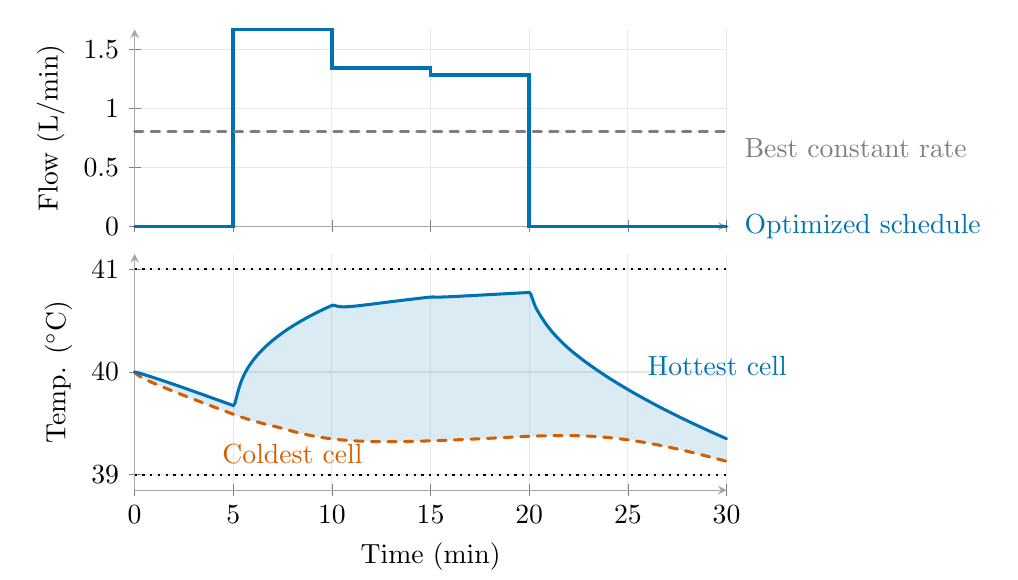
\begin{tikzpicture}
\begin{axis}[width=0.62\linewidth,
 height=2.5cm,
 scale only axis,
 xlabel={},
 ylabel={Flow (L/min)},
 axis lines=left,
 axis line style={gray!70},
 grid=major,
 grid style={gray!18},
 tick label style={font=\normalsize},
 label style={font=\normalsize},
 every axis plot/.append style={line cap=round},
 clip=false,
 xmin=0,
 xmax=30,
 ymin=0,
 scale only axis,name=top,xticklabels={}]
\addplot[color=main,line width=1.3pt,no marks,forget plot] coordinates {(0,4.64083e-12) (5,4.64083e-12) (5,1.66811) (10,1.66811) (10,1.34344) (15,1.34344) (15,1.28387) (20,1.28387) (20,1.07042e-12) (25,1.07042e-12) (25,1.06639e-12) (30,1.06639e-12)};
\addplot[color=muted,line width=1.1pt,dashed,no marks,forget plot] coordinates {(0,0.804748) (30,0.804748)};
\node[anchor=west,font=\normalsize,text=main,xshift=3pt,yshift=0pt] at (axis cs:30,1.06639e-12) {Optimized schedule};
\node[anchor=west,font=\normalsize,text=muted,xshift=3pt,yshift=-6pt] at (axis cs:30,0.804748) {Best constant rate};
\end{axis}
\begin{axis}[width=0.62\linewidth,
 height=3.0cm,
 scale only axis,
 xlabel={Time (min)},
 ylabel={Temp. ($^\circ$C)},
 axis lines=left,
 axis line style={gray!70},
 grid=major,
 grid style={gray!18},
 tick label style={font=\normalsize},
 label style={font=\normalsize},
 every axis plot/.append style={line cap=round},
 clip=false,
 xmin=0,
 xmax=30,
 ymin=38.85,
 ymax=41.15,
 scale only axis,at={(top.south)},anchor=north,yshift=-0.35cm]
\addplot[name path=lo1,draw=none,forget plot] coordinates {(0,40) (0.0833333,39.9833) (0.166667,39.9703) (0.25,39.9594) (0.333333,39.9497) (0.416667,39.9408) (0.5,39.9325) (0.583333,39.9245) (0.666667,39.9169) (0.75,39.9095) (0.833333,39.9023) (0.916667,39.8952) (1,39.8882) (1.08333,39.8813) (1.16667,39.8745) (1.25,39.8678) (1.33333,39.8611) (1.41667,39.8544) (1.5,39.8479) (1.58333,39.8413) (1.66667,39.8348) (1.75,39.8284) (1.83333,39.8219) (1.91667,39.8155) (2,39.8092) (2.08333,39.8028) (2.16667,39.7965) (2.25,39.7902) (2.33333,39.7839) (2.41667,39.7776) (2.5,39.7714) (2.58333,39.7652) (2.66667,39.7589) (2.75,39.7527) (2.83333,39.7466) (2.91667,39.7404) (3,39.7342) (3.08333,39.7281) (3.16667,39.722) (3.25,39.7158) (3.33333,39.7097) (3.41667,39.7036) (3.5,39.6975) (3.58333,39.6914) (3.66667,39.6854) (3.75,39.6793) (3.83333,39.6732) (3.91667,39.6672) (4,39.6611) (4.08333,39.6551) (4.16667,39.6491) (4.25,39.6431) (4.33333,39.637) (4.41667,39.631) (4.5,39.625) (4.58333,39.619) (4.66667,39.613) (4.75,39.607) (4.83333,39.601) (4.91667,39.5951) (5,39.5891) (5.08333,39.5832) (5.16667,39.5774) (5.25,39.5717) (5.33333,39.5661) (5.41667,39.5605) (5.5,39.5552) (5.58333,39.55) (5.66667,39.545) (5.75,39.5403) (5.83333,39.5358) (5.91667,39.5316) (6,39.5277) (6.08333,39.5229) (6.16667,39.5177) (6.25,39.5127) (6.33333,39.5079) (6.41667,39.5032) (6.5,39.4986) (6.58333,39.4942) (6.66667,39.49) (6.75,39.486) (6.83333,39.4821) (6.91667,39.4783) (7,39.4748) (7.08333,39.4713) (7.16667,39.4681) (7.25,39.4636) (7.33333,39.459) (7.41667,39.4545) (7.5,39.4502) (7.58333,39.446) (7.66667,39.4418) (7.75,39.437) (7.83333,39.4324) (7.91667,39.4279) (8,39.4235) (8.08333,39.4191) (8.16667,39.4149) (8.25,39.4108) (8.33333,39.4068) (8.41667,39.4029) (8.5,39.3992) (8.58333,39.3955) (8.66667,39.3919) (8.75,39.3885) (8.83333,39.3851) (8.91667,39.3819) (9,39.3787) (9.08333,39.3757) (9.16667,39.3728) (9.25,39.3699) (9.33333,39.3672) (9.41667,39.3646) (9.5,39.3621) (9.58333,39.3597) (9.66667,39.3573) (9.75,39.3551) (9.83333,39.353) (9.91667,39.3509) (10,39.349) (10.0833,39.3471) (10.1667,39.3453) (10.25,39.3436) (10.3333,39.3419) (10.4167,39.3403) (10.5,39.3388) (10.5833,39.3374) (10.6667,39.336) (10.75,39.3348) (10.8333,39.3336) (10.9167,39.3324) (11,39.3314) (11.0833,39.3304) (11.1667,39.3294) (11.25,39.3286) (11.3333,39.3277) (11.4167,39.327) (11.5,39.3263) (11.5833,39.3257) (11.6667,39.3251) (11.75,39.3246) (11.8333,39.3241) (11.9167,39.3237) (12,39.3233) (12.0833,39.3229) (12.1667,39.3226) (12.25,39.3224) (12.3333,39.3222) (12.4167,39.322) (12.5,39.3218) (12.5833,39.3217) (12.6667,39.3217) (12.75,39.3216) (12.8333,39.3216) (12.9167,39.3217) (13,39.3217) (13.0833,39.3218) (13.1667,39.3219) (13.25,39.322) (13.3333,39.3222) (13.4167,39.3224) (13.5,39.3226) (13.5833,39.3228) (13.6667,39.3231) (13.75,39.3234) (13.8333,39.3237) (13.9167,39.324) (14,39.3243) (14.0833,39.3247) (14.1667,39.3251) (14.25,39.3255) (14.3333,39.3259) (14.4167,39.3263) (14.5,39.3268) (14.5833,39.3272) (14.6667,39.3277) (14.75,39.3282) (14.8333,39.3287) (14.9167,39.3293) (15,39.3298) (15.0833,39.3303) (15.1667,39.3309) (15.25,39.3315) (15.3333,39.332) (15.4167,39.3326) (15.5,39.3332) (15.5833,39.3338) (15.6667,39.3344) (15.75,39.3351) (15.8333,39.3357) (15.9167,39.3364) (16,39.337) (16.0833,39.3377) (16.1667,39.3384) (16.25,39.339) (16.3333,39.3397) (16.4167,39.3404) (16.5,39.3411) (16.5833,39.3419) (16.6667,39.3426) (16.75,39.3433) (16.8333,39.344) (16.9167,39.3448) (17,39.3455) (17.0833,39.3463) (17.1667,39.347) (17.25,39.3478) (17.3333,39.3485) (17.4167,39.3493) (17.5,39.3501) (17.5833,39.3509) (17.6667,39.3516) (17.75,39.3524) (17.8333,39.3532) (17.9167,39.354) (18,39.3548) (18.0833,39.3556) (18.1667,39.3564) (18.25,39.3572) (18.3333,39.358) (18.4167,39.3588) (18.5,39.3596) (18.5833,39.3604) (18.6667,39.3612) (18.75,39.362) (18.8333,39.3628) (18.9167,39.3636) (19,39.3644) (19.0833,39.3653) (19.1667,39.3661) (19.25,39.3669) (19.3333,39.3677) (19.4167,39.3685) (19.5,39.3693) (19.5833,39.3702) (19.6667,39.371) (19.75,39.3718) (19.8333,39.3726) (19.9167,39.3735) (20,39.3743) (20.0833,39.3749) (20.1667,39.3755) (20.25,39.376) (20.3333,39.3764) (20.4167,39.3768) (20.5,39.3773) (20.5833,39.3776) (20.6667,39.378) (20.75,39.3784) (20.8333,39.3787) (20.9167,39.379) (21,39.3793) (21.0833,39.3796) (21.1667,39.3799) (21.25,39.3801) (21.3333,39.3803) (21.4167,39.3805) (21.5,39.3806) (21.5833,39.3807) (21.6667,39.3808) (21.75,39.3808) (21.8333,39.3808) (21.9167,39.3808) (22,39.3807) (22.0833,39.3805) (22.1667,39.3804) (22.25,39.3801) (22.3333,39.3798) (22.4167,39.3795) (22.5,39.3791) (22.5833,39.3787) (22.6667,39.3782) (22.75,39.3776) (22.8333,39.377) (22.9167,39.3763) (23,39.3756) (23.0833,39.3748) (23.1667,39.3739) (23.25,39.373) (23.3333,39.372) (23.4167,39.371) (23.5,39.3698) (23.5833,39.3687) (23.6667,39.3674) (23.75,39.3661) (23.8333,39.3647) (23.9167,39.3633) (24,39.3618) (24.0833,39.3603) (24.1667,39.3587) (24.25,39.357) (24.3333,39.3552) (24.4167,39.3534) (24.5,39.3516) (24.5833,39.3497) (24.6667,39.3477) (24.75,39.3457) (24.8333,39.3436) (24.9167,39.3414) (25,39.3392) (25.0833,39.337) (25.1667,39.3346) (25.25,39.3323) (25.3333,39.3299) (25.4167,39.3274) (25.5,39.3249) (25.5833,39.3223) (25.6667,39.3196) (25.75,39.317) (25.8333,39.3142) (25.9167,39.3115) (26,39.3086) (26.0833,39.3058) (26.1667,39.3029) (26.25,39.2999) (26.3333,39.2969) (26.4167,39.2938) (26.5,39.2907) (26.5833,39.2876) (26.6667,39.2844) (26.75,39.2812) (26.8333,39.278) (26.9167,39.2747) (27,39.2713) (27.0833,39.2679) (27.1667,39.2645) (27.25,39.2611) (27.3333,39.2576) (27.4167,39.2541) (27.5,39.2505) (27.5833,39.2469) (27.6667,39.2433) (27.75,39.2396) (27.8333,39.2359) (27.9167,39.2322) (28,39.2284) (28.0833,39.2246) (28.1667,39.2208) (28.25,39.217) (28.3333,39.2131) (28.4167,39.2092) (28.5,39.2052) (28.5833,39.2013) (28.6667,39.1973) (28.75,39.1933) (28.8333,39.1892) (28.9167,39.1851) (29,39.181) (29.0833,39.1769) (29.1667,39.1728) (29.25,39.1686) (29.3333,39.1644) (29.4167,39.1602) (29.5,39.1559) (29.5833,39.1517) (29.6667,39.1474) (29.75,39.1431) (29.8333,39.1387) (29.9167,39.1344) (30,39.13)};
\addplot[name path=hi1,draw=none,forget plot] coordinates {(0,40) (0.0833333,39.9967) (0.166667,39.9928) (0.25,39.9883) (0.333333,39.9836) (0.416667,39.9787) (0.5,39.9738) (0.583333,39.9688) (0.666667,39.9638) (0.75,39.9587) (0.833333,39.9536) (0.916667,39.9484) (1,39.9432) (1.08333,39.938) (1.16667,39.9327) (1.25,39.9274) (1.33333,39.9221) (1.41667,39.9167) (1.5,39.9113) (1.58333,39.9059) (1.66667,39.9005) (1.75,39.895) (1.83333,39.8896) (1.91667,39.884) (2,39.8785) (2.08333,39.873) (2.16667,39.8674) (2.25,39.8619) (2.33333,39.8563) (2.41667,39.8507) (2.5,39.8451) (2.58333,39.8394) (2.66667,39.8338) (2.75,39.8282) (2.83333,39.8225) (2.91667,39.8168) (3,39.8112) (3.08333,39.8055) (3.16667,39.7998) (3.25,39.7941) (3.33333,39.7884) (3.41667,39.7827) (3.5,39.777) (3.58333,39.7712) (3.66667,39.7655) (3.75,39.7598) (3.83333,39.7541) (3.91667,39.7483) (4,39.7426) (4.08333,39.7368) (4.16667,39.7311) (4.25,39.7253) (4.33333,39.7196) (4.41667,39.7138) (4.5,39.7081) (4.58333,39.7023) (4.66667,39.6965) (4.75,39.6908) (4.83333,39.685) (4.91667,39.6792) (5,39.6735) (5.08333,39.6951) (5.16667,39.756) (5.25,39.8177) (5.33333,39.8705) (5.41667,39.915) (5.5,39.953) (5.58333,39.9862) (5.66667,40.0159) (5.75,40.0429) (5.83333,40.0677) (5.91667,40.0907) (6,40.1123) (6.08333,40.1327) (6.16667,40.152) (6.25,40.1705) (6.33333,40.1881) (6.41667,40.205) (6.5,40.2212) (6.58333,40.2369) (6.66667,40.2521) (6.75,40.2667) (6.83333,40.2809) (6.91667,40.2947) (7,40.3081) (7.08333,40.3211) (7.16667,40.3338) (7.25,40.3462) (7.33333,40.3583) (7.41667,40.3701) (7.5,40.3817) (7.58333,40.393) (7.66667,40.404) (7.75,40.4149) (7.83333,40.4255) (7.91667,40.4359) (8,40.4462) (8.08333,40.4562) (8.16667,40.4661) (8.25,40.4757) (8.33333,40.4853) (8.41667,40.4946) (8.5,40.5038) (8.58333,40.5129) (8.66667,40.5218) (8.75,40.5306) (8.83333,40.5392) (8.91667,40.5478) (9,40.5561) (9.08333,40.5644) (9.16667,40.5726) (9.25,40.5806) (9.33333,40.5885) (9.41667,40.5963) (9.5,40.6041) (9.58333,40.6117) (9.66667,40.6192) (9.75,40.6266) (9.83333,40.6339) (9.91667,40.6411) (10,40.6482) (10.0833,40.6507) (10.1667,40.6462) (10.25,40.6415) (10.3333,40.6381) (10.4167,40.636) (10.5,40.6349) (10.5833,40.6346) (10.6667,40.6348) (10.75,40.6353) (10.8333,40.6362) (10.9167,40.6373) (11,40.6386) (11.0833,40.6401) (11.1667,40.6416) (11.25,40.6433) (11.3333,40.645) (11.4167,40.6468) (11.5,40.6486) (11.5833,40.6505) (11.6667,40.6524) (11.75,40.6544) (11.8333,40.6563) (11.9167,40.6583) (12,40.6603) (12.0833,40.6624) (12.1667,40.6644) (12.25,40.6664) (12.3333,40.6684) (12.4167,40.6705) (12.5,40.6725) (12.5833,40.6745) (12.6667,40.6766) (12.75,40.6786) (12.8333,40.6806) (12.9167,40.6826) (13,40.6846) (13.0833,40.6866) (13.1667,40.6886) (13.25,40.6906) (13.3333,40.6925) (13.4167,40.6945) (13.5,40.6964) (13.5833,40.6983) (13.6667,40.7003) (13.75,40.7022) (13.8333,40.7041) (13.9167,40.706) (14,40.7078) (14.0833,40.7097) (14.1667,40.7116) (14.25,40.7134) (14.3333,40.7152) (14.4167,40.7171) (14.5,40.7189) (14.5833,40.7207) (14.6667,40.7224) (14.75,40.7242) (14.8333,40.726) (14.9167,40.7277) (15,40.7295) (15.0833,40.7303) (15.1667,40.73) (15.25,40.7295) (15.3333,40.7294) (15.4167,40.7294) (15.5,40.7297) (15.5833,40.7301) (15.6667,40.7306) (15.75,40.7312) (15.8333,40.7318) (15.9167,40.7325) (16,40.7332) (16.0833,40.7339) (16.1667,40.7347) (16.25,40.7355) (16.3333,40.7363) (16.4167,40.7371) (16.5,40.7379) (16.5833,40.7388) (16.6667,40.7396) (16.75,40.7405) (16.8333,40.7413) (16.9167,40.7422) (17,40.743) (17.0833,40.7439) (17.1667,40.7448) (17.25,40.7457) (17.3333,40.7465) (17.4167,40.7474) (17.5,40.7483) (17.5833,40.7492) (17.6667,40.75) (17.75,40.7509) (17.8333,40.7518) (17.9167,40.7527) (18,40.7536) (18.0833,40.7544) (18.1667,40.7553) (18.25,40.7562) (18.3333,40.7571) (18.4167,40.7579) (18.5,40.7588) (18.5833,40.7597) (18.6667,40.7606) (18.75,40.7614) (18.8333,40.7623) (18.9167,40.7632) (19,40.764) (19.0833,40.7649) (19.1667,40.7658) (19.25,40.7666) (19.3333,40.7675) (19.4167,40.7683) (19.5,40.7692) (19.5833,40.77) (19.6667,40.7709) (19.75,40.7717) (19.8333,40.7726) (19.9167,40.7734) (20,40.7743) (20.0833,40.7566) (20.1667,40.7116) (20.25,40.665) (20.3333,40.6258) (20.4167,40.5979) (20.5,40.5706) (20.5833,40.5442) (20.6667,40.5189) (20.75,40.4948) (20.8333,40.4719) (20.9167,40.45) (21,40.4291) (21.0833,40.4091) (21.1667,40.3899) (21.25,40.3714) (21.3333,40.3536) (21.4167,40.3364) (21.5,40.3197) (21.5833,40.3035) (21.6667,40.2877) (21.75,40.2724) (21.8333,40.2575) (21.9167,40.2429) (22,40.2286) (22.0833,40.2146) (22.1667,40.2012) (22.25,40.188) (22.3333,40.1751) (22.4167,40.1623) (22.5,40.1498) (22.5833,40.1374) (22.6667,40.1251) (22.75,40.1131) (22.8333,40.1011) (22.9167,40.0894) (23,40.0777) (23.0833,40.0662) (23.1667,40.0549) (23.25,40.0436) (23.3333,40.0325) (23.4167,40.0215) (23.5,40.0106) (23.5833,39.9998) (23.6667,39.989) (23.75,39.9784) (23.8333,39.9679) (23.9167,39.9575) (24,39.9472) (24.0833,39.937) (24.1667,39.9268) (24.25,39.9168) (24.3333,39.9068) (24.4167,39.8969) (24.5,39.887) (24.5833,39.8773) (24.6667,39.8676) (24.75,39.858) (24.8333,39.8485) (24.9167,39.839) (25,39.8296) (25.0833,39.8203) (25.1667,39.811) (25.25,39.8018) (25.3333,39.7926) (25.4167,39.7835) (25.5,39.7745) (25.5833,39.7655) (25.6667,39.7566) (25.75,39.7477) (25.8333,39.7389) (25.9167,39.7302) (26,39.7215) (26.0833,39.7128) (26.1667,39.7042) (26.25,39.6957) (26.3333,39.6872) (26.4167,39.6787) (26.5,39.6703) (26.5833,39.6619) (26.6667,39.6536) (26.75,39.6453) (26.8333,39.6371) (26.9167,39.6289) (27,39.6208) (27.0833,39.6126) (27.1667,39.6046) (27.25,39.5966) (27.3333,39.5886) (27.4167,39.5806) (27.5,39.5727) (27.5833,39.5648) (27.6667,39.557) (27.75,39.5492) (27.8333,39.5414) (27.9167,39.5337) (28,39.526) (28.0833,39.5184) (28.1667,39.5107) (28.25,39.5031) (28.3333,39.4956) (28.4167,39.488) (28.5,39.4805) (28.5833,39.4731) (28.6667,39.4656) (28.75,39.4582) (28.8333,39.4509) (28.9167,39.4435) (29,39.4362) (29.0833,39.4289) (29.1667,39.4216) (29.25,39.4144) (29.3333,39.4072) (29.4167,39.4) (29.5,39.3928) (29.5833,39.3857) (29.6667,39.3786) (29.75,39.3715) (29.8333,39.3644) (29.9167,39.3574) (30,39.3504)};
\addplot[fill=main,fill opacity=0.14,forget plot] fill between[of=lo1 and hi1];
\addplot[color=accent,line width=1.1pt,dashed,no marks,forget plot] coordinates {(0,40) (0.0833333,39.9833) (0.166667,39.9703) (0.25,39.9594) (0.333333,39.9497) (0.416667,39.9408) (0.5,39.9325) (0.583333,39.9245) (0.666667,39.9169) (0.75,39.9095) (0.833333,39.9023) (0.916667,39.8952) (1,39.8882) (1.08333,39.8813) (1.16667,39.8745) (1.25,39.8678) (1.33333,39.8611) (1.41667,39.8544) (1.5,39.8479) (1.58333,39.8413) (1.66667,39.8348) (1.75,39.8284) (1.83333,39.8219) (1.91667,39.8155) (2,39.8092) (2.08333,39.8028) (2.16667,39.7965) (2.25,39.7902) (2.33333,39.7839) (2.41667,39.7776) (2.5,39.7714) (2.58333,39.7652) (2.66667,39.7589) (2.75,39.7527) (2.83333,39.7466) (2.91667,39.7404) (3,39.7342) (3.08333,39.7281) (3.16667,39.722) (3.25,39.7158) (3.33333,39.7097) (3.41667,39.7036) (3.5,39.6975) (3.58333,39.6914) (3.66667,39.6854) (3.75,39.6793) (3.83333,39.6732) (3.91667,39.6672) (4,39.6611) (4.08333,39.6551) (4.16667,39.6491) (4.25,39.6431) (4.33333,39.637) (4.41667,39.631) (4.5,39.625) (4.58333,39.619) (4.66667,39.613) (4.75,39.607) (4.83333,39.601) (4.91667,39.5951) (5,39.5891) (5.08333,39.5832) (5.16667,39.5774) (5.25,39.5717) (5.33333,39.5661) (5.41667,39.5605) (5.5,39.5552) (5.58333,39.55) (5.66667,39.545) (5.75,39.5403) (5.83333,39.5358) (5.91667,39.5316) (6,39.5277) (6.08333,39.5229) (6.16667,39.5177) (6.25,39.5127) (6.33333,39.5079) (6.41667,39.5032) (6.5,39.4986) (6.58333,39.4942) (6.66667,39.49) (6.75,39.486) (6.83333,39.4821) (6.91667,39.4783) (7,39.4748) (7.08333,39.4713) (7.16667,39.4681) (7.25,39.4636) (7.33333,39.459) (7.41667,39.4545) (7.5,39.4502) (7.58333,39.446) (7.66667,39.4418) (7.75,39.437) (7.83333,39.4324) (7.91667,39.4279) (8,39.4235) (8.08333,39.4191) (8.16667,39.4149) (8.25,39.4108) (8.33333,39.4068) (8.41667,39.4029) (8.5,39.3992) (8.58333,39.3955) (8.66667,39.3919) (8.75,39.3885) (8.83333,39.3851) (8.91667,39.3819) (9,39.3787) (9.08333,39.3757) (9.16667,39.3728) (9.25,39.3699) (9.33333,39.3672) (9.41667,39.3646) (9.5,39.3621) (9.58333,39.3597) (9.66667,39.3573) (9.75,39.3551) (9.83333,39.353) (9.91667,39.3509) (10,39.349) (10.0833,39.3471) (10.1667,39.3453) (10.25,39.3436) (10.3333,39.3419) (10.4167,39.3403) (10.5,39.3388) (10.5833,39.3374) (10.6667,39.336) (10.75,39.3348) (10.8333,39.3336) (10.9167,39.3324) (11,39.3314) (11.0833,39.3304) (11.1667,39.3294) (11.25,39.3286) (11.3333,39.3277) (11.4167,39.327) (11.5,39.3263) (11.5833,39.3257) (11.6667,39.3251) (11.75,39.3246) (11.8333,39.3241) (11.9167,39.3237) (12,39.3233) (12.0833,39.3229) (12.1667,39.3226) (12.25,39.3224) (12.3333,39.3222) (12.4167,39.322) (12.5,39.3218) (12.5833,39.3217) (12.6667,39.3217) (12.75,39.3216) (12.8333,39.3216) (12.9167,39.3217) (13,39.3217) (13.0833,39.3218) (13.1667,39.3219) (13.25,39.322) (13.3333,39.3222) (13.4167,39.3224) (13.5,39.3226) (13.5833,39.3228) (13.6667,39.3231) (13.75,39.3234) (13.8333,39.3237) (13.9167,39.324) (14,39.3243) (14.0833,39.3247) (14.1667,39.3251) (14.25,39.3255) (14.3333,39.3259) (14.4167,39.3263) (14.5,39.3268) (14.5833,39.3272) (14.6667,39.3277) (14.75,39.3282) (14.8333,39.3287) (14.9167,39.3293) (15,39.3298) (15.0833,39.3303) (15.1667,39.3309) (15.25,39.3315) (15.3333,39.332) (15.4167,39.3326) (15.5,39.3332) (15.5833,39.3338) (15.6667,39.3344) (15.75,39.3351) (15.8333,39.3357) (15.9167,39.3364) (16,39.337) (16.0833,39.3377) (16.1667,39.3384) (16.25,39.339) (16.3333,39.3397) (16.4167,39.3404) (16.5,39.3411) (16.5833,39.3419) (16.6667,39.3426) (16.75,39.3433) (16.8333,39.344) (16.9167,39.3448) (17,39.3455) (17.0833,39.3463) (17.1667,39.347) (17.25,39.3478) (17.3333,39.3485) (17.4167,39.3493) (17.5,39.3501) (17.5833,39.3509) (17.6667,39.3516) (17.75,39.3524) (17.8333,39.3532) (17.9167,39.354) (18,39.3548) (18.0833,39.3556) (18.1667,39.3564) (18.25,39.3572) (18.3333,39.358) (18.4167,39.3588) (18.5,39.3596) (18.5833,39.3604) (18.6667,39.3612) (18.75,39.362) (18.8333,39.3628) (18.9167,39.3636) (19,39.3644) (19.0833,39.3653) (19.1667,39.3661) (19.25,39.3669) (19.3333,39.3677) (19.4167,39.3685) (19.5,39.3693) (19.5833,39.3702) (19.6667,39.371) (19.75,39.3718) (19.8333,39.3726) (19.9167,39.3735) (20,39.3743) (20.0833,39.3749) (20.1667,39.3755) (20.25,39.376) (20.3333,39.3764) (20.4167,39.3768) (20.5,39.3773) (20.5833,39.3776) (20.6667,39.378) (20.75,39.3784) (20.8333,39.3787) (20.9167,39.379) (21,39.3793) (21.0833,39.3796) (21.1667,39.3799) (21.25,39.3801) (21.3333,39.3803) (21.4167,39.3805) (21.5,39.3806) (21.5833,39.3807) (21.6667,39.3808) (21.75,39.3808) (21.8333,39.3808) (21.9167,39.3808) (22,39.3807) (22.0833,39.3805) (22.1667,39.3804) (22.25,39.3801) (22.3333,39.3798) (22.4167,39.3795) (22.5,39.3791) (22.5833,39.3787) (22.6667,39.3782) (22.75,39.3776) (22.8333,39.377) (22.9167,39.3763) (23,39.3756) (23.0833,39.3748) (23.1667,39.3739) (23.25,39.373) (23.3333,39.372) (23.4167,39.371) (23.5,39.3698) (23.5833,39.3687) (23.6667,39.3674) (23.75,39.3661) (23.8333,39.3647) (23.9167,39.3633) (24,39.3618) (24.0833,39.3603) (24.1667,39.3587) (24.25,39.357) (24.3333,39.3552) (24.4167,39.3534) (24.5,39.3516) (24.5833,39.3497) (24.6667,39.3477) (24.75,39.3457) (24.8333,39.3436) (24.9167,39.3414) (25,39.3392) (25.0833,39.337) (25.1667,39.3346) (25.25,39.3323) (25.3333,39.3299) (25.4167,39.3274) (25.5,39.3249) (25.5833,39.3223) (25.6667,39.3196) (25.75,39.317) (25.8333,39.3142) (25.9167,39.3115) (26,39.3086) (26.0833,39.3058) (26.1667,39.3029) (26.25,39.2999) (26.3333,39.2969) (26.4167,39.2938) (26.5,39.2907) (26.5833,39.2876) (26.6667,39.2844) (26.75,39.2812) (26.8333,39.278) (26.9167,39.2747) (27,39.2713) (27.0833,39.2679) (27.1667,39.2645) (27.25,39.2611) (27.3333,39.2576) (27.4167,39.2541) (27.5,39.2505) (27.5833,39.2469) (27.6667,39.2433) (27.75,39.2396) (27.8333,39.2359) (27.9167,39.2322) (28,39.2284) (28.0833,39.2246) (28.1667,39.2208) (28.25,39.217) (28.3333,39.2131) (28.4167,39.2092) (28.5,39.2052) (28.5833,39.2013) (28.6667,39.1973) (28.75,39.1933) (28.8333,39.1892) (28.9167,39.1851) (29,39.181) (29.0833,39.1769) (29.1667,39.1728) (29.25,39.1686) (29.3333,39.1644) (29.4167,39.1602) (29.5,39.1559) (29.5833,39.1517) (29.6667,39.1474) (29.75,39.1431) (29.8333,39.1387) (29.9167,39.1344) (30,39.13)};
\addplot[color=main,line width=1.1pt,no marks,forget plot] coordinates {(0,40) (0.0833333,39.9967) (0.166667,39.9928) (0.25,39.9883) (0.333333,39.9836) (0.416667,39.9787) (0.5,39.9738) (0.583333,39.9688) (0.666667,39.9638) (0.75,39.9587) (0.833333,39.9536) (0.916667,39.9484) (1,39.9432) (1.08333,39.938) (1.16667,39.9327) (1.25,39.9274) (1.33333,39.9221) (1.41667,39.9167) (1.5,39.9113) (1.58333,39.9059) (1.66667,39.9005) (1.75,39.895) (1.83333,39.8896) (1.91667,39.884) (2,39.8785) (2.08333,39.873) (2.16667,39.8674) (2.25,39.8619) (2.33333,39.8563) (2.41667,39.8507) (2.5,39.8451) (2.58333,39.8394) (2.66667,39.8338) (2.75,39.8282) (2.83333,39.8225) (2.91667,39.8168) (3,39.8112) (3.08333,39.8055) (3.16667,39.7998) (3.25,39.7941) (3.33333,39.7884) (3.41667,39.7827) (3.5,39.777) (3.58333,39.7712) (3.66667,39.7655) (3.75,39.7598) (3.83333,39.7541) (3.91667,39.7483) (4,39.7426) (4.08333,39.7368) (4.16667,39.7311) (4.25,39.7253) (4.33333,39.7196) (4.41667,39.7138) (4.5,39.7081) (4.58333,39.7023) (4.66667,39.6965) (4.75,39.6908) (4.83333,39.685) (4.91667,39.6792) (5,39.6735) (5.08333,39.6951) (5.16667,39.756) (5.25,39.8177) (5.33333,39.8705) (5.41667,39.915) (5.5,39.953) (5.58333,39.9862) (5.66667,40.0159) (5.75,40.0429) (5.83333,40.0677) (5.91667,40.0907) (6,40.1123) (6.08333,40.1327) (6.16667,40.152) (6.25,40.1705) (6.33333,40.1881) (6.41667,40.205) (6.5,40.2212) (6.58333,40.2369) (6.66667,40.2521) (6.75,40.2667) (6.83333,40.2809) (6.91667,40.2947) (7,40.3081) (7.08333,40.3211) (7.16667,40.3338) (7.25,40.3462) (7.33333,40.3583) (7.41667,40.3701) (7.5,40.3817) (7.58333,40.393) (7.66667,40.404) (7.75,40.4149) (7.83333,40.4255) (7.91667,40.4359) (8,40.4462) (8.08333,40.4562) (8.16667,40.4661) (8.25,40.4757) (8.33333,40.4853) (8.41667,40.4946) (8.5,40.5038) (8.58333,40.5129) (8.66667,40.5218) (8.75,40.5306) (8.83333,40.5392) (8.91667,40.5478) (9,40.5561) (9.08333,40.5644) (9.16667,40.5726) (9.25,40.5806) (9.33333,40.5885) (9.41667,40.5963) (9.5,40.6041) (9.58333,40.6117) (9.66667,40.6192) (9.75,40.6266) (9.83333,40.6339) (9.91667,40.6411) (10,40.6482) (10.0833,40.6507) (10.1667,40.6462) (10.25,40.6415) (10.3333,40.6381) (10.4167,40.636) (10.5,40.6349) (10.5833,40.6346) (10.6667,40.6348) (10.75,40.6353) (10.8333,40.6362) (10.9167,40.6373) (11,40.6386) (11.0833,40.6401) (11.1667,40.6416) (11.25,40.6433) (11.3333,40.645) (11.4167,40.6468) (11.5,40.6486) (11.5833,40.6505) (11.6667,40.6524) (11.75,40.6544) (11.8333,40.6563) (11.9167,40.6583) (12,40.6603) (12.0833,40.6624) (12.1667,40.6644) (12.25,40.6664) (12.3333,40.6684) (12.4167,40.6705) (12.5,40.6725) (12.5833,40.6745) (12.6667,40.6766) (12.75,40.6786) (12.8333,40.6806) (12.9167,40.6826) (13,40.6846) (13.0833,40.6866) (13.1667,40.6886) (13.25,40.6906) (13.3333,40.6925) (13.4167,40.6945) (13.5,40.6964) (13.5833,40.6983) (13.6667,40.7003) (13.75,40.7022) (13.8333,40.7041) (13.9167,40.706) (14,40.7078) (14.0833,40.7097) (14.1667,40.7116) (14.25,40.7134) (14.3333,40.7152) (14.4167,40.7171) (14.5,40.7189) (14.5833,40.7207) (14.6667,40.7224) (14.75,40.7242) (14.8333,40.726) (14.9167,40.7277) (15,40.7295) (15.0833,40.7303) (15.1667,40.73) (15.25,40.7295) (15.3333,40.7294) (15.4167,40.7294) (15.5,40.7297) (15.5833,40.7301) (15.6667,40.7306) (15.75,40.7312) (15.8333,40.7318) (15.9167,40.7325) (16,40.7332) (16.0833,40.7339) (16.1667,40.7347) (16.25,40.7355) (16.3333,40.7363) (16.4167,40.7371) (16.5,40.7379) (16.5833,40.7388) (16.6667,40.7396) (16.75,40.7405) (16.8333,40.7413) (16.9167,40.7422) (17,40.743) (17.0833,40.7439) (17.1667,40.7448) (17.25,40.7457) (17.3333,40.7465) (17.4167,40.7474) (17.5,40.7483) (17.5833,40.7492) (17.6667,40.75) (17.75,40.7509) (17.8333,40.7518) (17.9167,40.7527) (18,40.7536) (18.0833,40.7544) (18.1667,40.7553) (18.25,40.7562) (18.3333,40.7571) (18.4167,40.7579) (18.5,40.7588) (18.5833,40.7597) (18.6667,40.7606) (18.75,40.7614) (18.8333,40.7623) (18.9167,40.7632) (19,40.764) (19.0833,40.7649) (19.1667,40.7658) (19.25,40.7666) (19.3333,40.7675) (19.4167,40.7683) (19.5,40.7692) (19.5833,40.77) (19.6667,40.7709) (19.75,40.7717) (19.8333,40.7726) (19.9167,40.7734) (20,40.7743) (20.0833,40.7566) (20.1667,40.7116) (20.25,40.665) (20.3333,40.6258) (20.4167,40.5979) (20.5,40.5706) (20.5833,40.5442) (20.6667,40.5189) (20.75,40.4948) (20.8333,40.4719) (20.9167,40.45) (21,40.4291) (21.0833,40.4091) (21.1667,40.3899) (21.25,40.3714) (21.3333,40.3536) (21.4167,40.3364) (21.5,40.3197) (21.5833,40.3035) (21.6667,40.2877) (21.75,40.2724) (21.8333,40.2575) (21.9167,40.2429) (22,40.2286) (22.0833,40.2146) (22.1667,40.2012) (22.25,40.188) (22.3333,40.1751) (22.4167,40.1623) (22.5,40.1498) (22.5833,40.1374) (22.6667,40.1251) (22.75,40.1131) (22.8333,40.1011) (22.9167,40.0894) (23,40.0777) (23.0833,40.0662) (23.1667,40.0549) (23.25,40.0436) (23.3333,40.0325) (23.4167,40.0215) (23.5,40.0106) (23.5833,39.9998) (23.6667,39.989) (23.75,39.9784) (23.8333,39.9679) (23.9167,39.9575) (24,39.9472) (24.0833,39.937) (24.1667,39.9268) (24.25,39.9168) (24.3333,39.9068) (24.4167,39.8969) (24.5,39.887) (24.5833,39.8773) (24.6667,39.8676) (24.75,39.858) (24.8333,39.8485) (24.9167,39.839) (25,39.8296) (25.0833,39.8203) (25.1667,39.811) (25.25,39.8018) (25.3333,39.7926) (25.4167,39.7835) (25.5,39.7745) (25.5833,39.7655) (25.6667,39.7566) (25.75,39.7477) (25.8333,39.7389) (25.9167,39.7302) (26,39.7215) (26.0833,39.7128) (26.1667,39.7042) (26.25,39.6957) (26.3333,39.6872) (26.4167,39.6787) (26.5,39.6703) (26.5833,39.6619) (26.6667,39.6536) (26.75,39.6453) (26.8333,39.6371) (26.9167,39.6289) (27,39.6208) (27.0833,39.6126) (27.1667,39.6046) (27.25,39.5966) (27.3333,39.5886) (27.4167,39.5806) (27.5,39.5727) (27.5833,39.5648) (27.6667,39.557) (27.75,39.5492) (27.8333,39.5414) (27.9167,39.5337) (28,39.526) (28.0833,39.5184) (28.1667,39.5107) (28.25,39.5031) (28.3333,39.4956) (28.4167,39.488) (28.5,39.4805) (28.5833,39.4731) (28.6667,39.4656) (28.75,39.4582) (28.8333,39.4509) (28.9167,39.4435) (29,39.4362) (29.0833,39.4289) (29.1667,39.4216) (29.25,39.4144) (29.3333,39.4072) (29.4167,39.4) (29.5,39.3928) (29.5833,39.3857) (29.6667,39.3786) (29.75,39.3715) (29.8333,39.3644) (29.9167,39.3574) (30,39.3504)};
\draw[black, line width=0.8pt, dotted] ({rel axis cs:0,0}|-{axis cs:0,39}) -- ({rel axis cs:1,0}|-{axis cs:0,39});
\draw[black, line width=0.8pt, dotted] ({rel axis cs:0,0}|-{axis cs:0,41}) -- ({rel axis cs:1,0}|-{axis cs:0,41});
\node[anchor=south west,font=\normalsize,text=main,xshift=0pt,yshift=0pt] at (axis cs:25.5,39.8745) {Hottest cell};
\node[anchor=north,font=\normalsize,text=accent,xshift=0pt,yshift=0pt] at (axis cs:8,39.3935) {Coldest cell};
\end{axis}
\end{tikzpicture}
\caption{Buffered six-segment replenishment}\label{fig:control}
\end{figure}
The accepted 6-segment policy is off for the first 5.0 minutes and last 10.0 minutes, with a peak flow of 1.67 L/min. For consecutive 5-minute intervals the rates, rounded to nine decimals, are 0, 1.668107192, 1.343440056, 1.283871597, 0, 0 L/min; the interval duration times their sum is 21.477094 L. It adds 21.48 L, 11.0\% below the constant rate. Its 0.1°C design margin sacrifices some water savings to protect the stated constraints. The remaining 6.06 L gap to the energy bound is not an optimality certificate.

The unbuffered 12-segment candidate uses 19.35 L but reaches a spread of 1.531°C on the finest mesh, above the 1.5°C limit, so it is rejected. Among the tested buffered alternatives, the accepted 6-segment policy gives spreads of 1.400, 1.395 and 1.416°C on the 8 × 4 × 3, 12 × 6 × 4 and 16 × 8 × 6 meshes. Independently integrated continuous-time bounds also pass on each mesh. This establishes numerical feasibility for these tested networks, not mesh-independent physics or a global minimum.

\subsection{Temperature–water trade-off}
The task asks for a bath close to its initial temperature without wasting much water, which is a trade-off rather than a single optimum. Figure \ref{fig:frontier} repeats the search while the allowed fall below 40°C changes from 0.25 to 3°C; the 1°C case is the baseline. With a fall of 2.5°C or more the stored heat suffices and no water is added. At 2°C the best constant rate adds 1.9 L, at 1.5°C 12.9 L, at 1°C 24.1 L and at 0.75°C 29.8 L. Between 2°C and 0.75°C each further 0.5°C of tolerance is therefore worth roughly 11 L, almost linearly. At 0.5°C the best constant rate adds 36.3 L; for a fall of 0.25°C no constant-rate policy was accepted, while the perfectly mixed bath would still need 30.7 L.

Figure \ref{fig:frontier} compares searched spatial policies with analytical benchmarks. Crosses denote unsuccessful searches; the dotted line marks the baseline.

\begin{figure}[ht]\centering
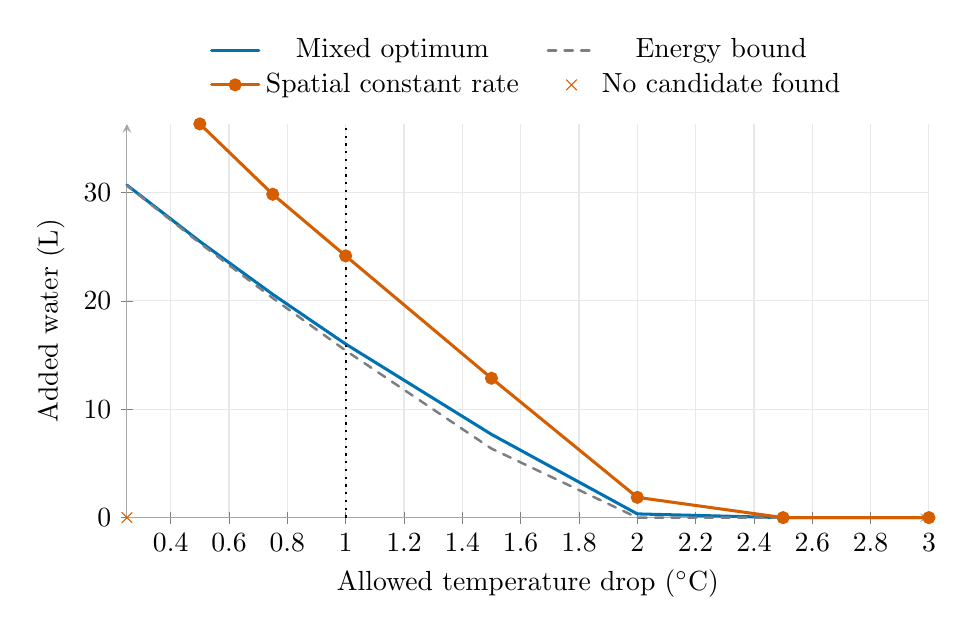
\begin{tikzpicture}
\begin{axis}[width=0.84\linewidth,
 height=5.0cm,
 scale only axis,
 xlabel={Allowed temperature drop ($^\circ$C)},
 ylabel={Added water (L)},
 axis lines=left,
 axis line style={gray!70},
 grid=major,
 grid style={gray!18},
 tick label style={font=\normalsize},
 label style={font=\normalsize},
 every axis plot/.append style={line cap=round},
 clip=false,
 legend style={font=\normalsize,draw=none,fill=none,at={(0.5,1.04)},anchor=south,/tikz/every even column/.append style={column sep=8pt},legend columns=2,}]
\addplot[color=main,line width=1.1pt,no marks] coordinates {(3,0) (2.5,0) (2,0.343176) (1.5,7.67938) (1,16.014) (0.75,20.5948) (0.5,25.475) (0.25,30.6749)};\addlegendentry{Mixed optimum}
\addplot[color=muted,line width=0.9pt,dashed,no marks] coordinates {(3,0) (2.5,0) (2,0) (1.5,6.36811) (1,15.4132) (0.75,20.2513) (0.5,25.3198) (0.25,30.6355)};\addlegendentry{Energy bound}
\addplot[color=accent,line width=1.1pt,mark=*,mark size=1.8pt] coordinates {(3,0) (2.5,0) (2,1.87033) (1.5,12.859) (1,24.1425) (0.75,29.8268) (0.5,36.3161)};\addlegendentry{Spatial constant rate}
\addplot[only marks,mark=x,mark size=2.6pt,color=accent] coordinates {(0.25,0)};\addlegendentry{No candidate found}
\draw[black, line width=0.8pt, dotted] ({axis cs:1,0}|-{rel axis cs:0,0}) -- ({axis cs:1,0}|-{rel axis cs:0,1});
\end{axis}
\end{tikzpicture}
\caption{Water use and temperature tolerance}\label{fig:frontier}
\end{figure}
The spatial-minus-mixed gap increases from 1.5 L at a 2°C fall to 9.2 L at 0.75°C. Scheduling lowers the baseline by 11\%; schedules at other tolerances were not optimized.

\subsection{Delivery-error sensitivity}
We distinguish fixed tap bias from random segment errors. For the unbuffered 12-segment candidate, multiplying every rate by 0.9 or 1.1 crosses a limit by 0.076 and 0.126°C. Independently drawing each multiplier from a normal distribution of mean 1 and standard deviation 0.1, clipped below zero, gives median and 5th-percentile slacks of -0.070 and -0.217°C (200 draws, seed 11). Standard deviation 0.1 does not mean an error bounded within ±10\%. Negative slack is a violation, however small.

The error is not symmetric. The most sensitive segment is segment 4 (2.81 L/min), where raising the flow by 20\% breaks the limits by 0.245°C and lowering it by 20\% by 0.047°C: extra hot water overheats the inlet region and widens the spread. Over-delivery in a high-flow segment is the error to guard against. 1 of the 5 active segments tolerates a 20\% error in either direction.

The price of a margin is measured on a 6-segment version. Requiring all three limits to hold with a buffer b gives 19.50 L at b = 0, 21.48 L (+10\%) at 0.1°C, 23.81 L (+22\%) at 0.2°C and 26.83 L (+38\%) at 0.3°C. With the 0.1°C buffer, 74\% of 200 draws with independent Gaussian multiplier standard deviation 0.1 stay within the limits. The 0.1°C policy is selected here for its independently checked numerical margin. Its 74\% acceptance under the stated random error model does not make it a reliable manual prescription; a real bath needs temperature feedback and separate calibration.

\subsection{Supply decisions from temperature probes}
Mixing changes timing: the weaker-mixing candidate starts immediately. Two probes miss violations in two of nine cases. We now propagate observation ambiguity into the supply decision.

A separate synthetic trial applies (0, 0, 1.2, 0, 0, 0) L/min in five-minute stages. Known geometry starts uniformly at 40°C; cells 89 and 6 are read every 30 s. Assumed reading errors and constant probe biases are each bounded by ±0.02°C; these are not instrument specifications.

For parameters $\theta$ and probe j, let $d_j(t;\theta)=T_j(t;\theta)-y_j(t)$. At observed times $\mathcal{T}=\{0,30,\ldots,1800\}$ s, a model is compatible when a constant correction $a_j$ exists such that

\begin{equation}\min_{|a_j|\leq0.02}\max_{t\in\mathcal{T}}|d_j(t;\theta)-a_j|\leq0.02\quad(j=1,2).\end{equation}
The extreme-discrepancy midpoint clipped to the bias bound is the minimax correction, with physical bias $b_j=-a_j$. A trace from -0.04 to +0.04°C fails: bias cannot vary between readings.

Our grid has 7 mixing values (0.00085–0.00115 m²/s), 9 surface and 9 body coefficients (20–30 and 15–35 W/(m² K)), and 5 delivery multipliers (0.95–1.05). Of 2835 models, 178 fit. This finite decision ambiguity set is neither a confidence region nor a probability distribution.

Table \ref{tab:measurement-control} compares archived policies with a replacement optimized on ten extreme/failing models, using a 2 L/min bound, 0.1°C target and 0.03°C extra floor reserve. All 178 pass three-grid envelopes; the tightest spread bound is 1.496828°C. The selected target is not an all-model margin or global optimum.

\begin{table}[ht]\centering\normalsize\caption{Policies on the same measurement-compatible set}\label{tab:measurement-control}
\begin{tabular}{@{}>{\raggedright\arraybackslash}p{0.3376\dimexpr\linewidth-6\tabcolsep\relax}>{\raggedright\arraybackslash}p{0.1838\dimexpr\linewidth-6\tabcolsep\relax}>{\raggedright\arraybackslash}p{0.2607\dimexpr\linewidth-6\tabcolsep\relax}>{\raggedright\arraybackslash}p{0.2179\dimexpr\linewidth-6\tabcolsep\relax}@{}}
\toprule
Policy & Command (L) & Delivered (L) & Sampled pass \\ \midrule
Constant & 24.14 & 22.94–25.35 & 130/178 \\
Nominal six-stage & 21.48 & 20.40–22.55 & 174/178 \\
Ambiguity-set six-stage & 23.48 & 22.31–24.66 & 178/178 \\ \bottomrule
\end{tabular}
\end{table}
The table uses the same 178 models and five-second sampling; archived policies were not re-optimized. Only the replacement has 534 three-grid envelopes. Its five-minute rates are 0.892820, 1.473786, 1.179268, 1.150408, 0.000000, 0.000000 L/min; envelope extrema are 39.1297/40.9238°C.

The replacement costs 9.33\% more than the nominal policy. A separate zero-inlet trial with the same prior, probes and errors retains 510 models, including unidentified delivery bias; its candidate passes 1530 three-grid envelopes. The two observation sets intersect in 167 models; they are not nested or probabilistic.

Table \ref{tab:information-cost} separates control and trial water. Both candidates restart at uniform 40°C with the same control family and design targets.

\begin{table}[ht]\centering\normalsize\caption{Observation-conditioned trial and control costs}\label{tab:information-cost}
\begin{tabular}{@{}>{\raggedright\arraybackslash}p{0.3846\dimexpr\linewidth-6\tabcolsep\relax}>{\raggedright\arraybackslash}p{0.1325\dimexpr\linewidth-6\tabcolsep\relax}>{\raggedright\arraybackslash}p{0.2650\dimexpr\linewidth-6\tabcolsep\relax}>{\raggedright\arraybackslash}p{0.2179\dimexpr\linewidth-6\tabcolsep\relax}@{}}
\toprule
Observation / trial & Models & Control (L) & Trial (L) \\ \midrule
Nominal / passive & 510 & 24.39 & 0.00 \\
Nominal / pulse & 178 & 23.48 & 6.00 \\ \bottomrule
\end{tabular}
\end{table}
Passive rates are 1.419252, 1.083923, 1.055204, 1.044908, 0.274962, 0.000000 L/min. Initial filling and reset are not free; these conditional candidates do not establish expected information value or global optimality.

Let n unchanged baths share one trial; let $\alpha\in[0.95,1.05]$ be the common delivery multiplier and $R_0,R_1$ the actual reset litres for passive and pulse designs. The difference between their total actual-water costs is

\begin{equation}C_0-C_1=\alpha\bigl(n\Delta-6\bigr)+R_0-R_1,\qquad \Delta=0.909836\ \mathrm{L}.\end{equation}
At nominal delivery, passive costs less for one bath if $R_0-R_1<5.0902$ L. Equal reset costs give a crossover at 6.59 baths: passive is cheaper through six, pulse from seven. Reuse requires unchanged geometry, heat transfer, probes and delivery bias; otherwise remeasure. This is not online feedback or a real-bath guarantee.

\section{Geometry and body-parameter sensitivity}
\begin{table}[ht]\centering\normalsize\caption{Geometry, size and body scenarios}\label{tab:8}
\begin{tabular}{@{}>{\raggedright\arraybackslash}p{0.3162\dimexpr\linewidth-4\tabcolsep\relax}>{\raggedright\arraybackslash}p{0.1838\dimexpr\linewidth-4\tabcolsep\relax}>{\raggedright\arraybackslash}p{0.5000\dimexpr\linewidth-4\tabcolsep\relax}@{}}
\toprule
Change from baseline & Water (L) & Interpretation \\ \midrule
Shallow Wide & No candidate & Same envelope volume \\
Deep Narrow & 17.48 & Same envelope volume \\
Small Bath & 27.05 & Lower water depth \\
Large Bath & 20.39 & Higher water depth \\
Deep Bath & 13.05 & Depth 0.35 m, like a bath filled to the shoulders \\
Larger Body & 28.11 & More displacement/contact \\
Long Body & 23.85 & Shape only; fixed volume/area \\
Warmer Skin & 21.08 & Skin at 36°C \\
Cooler Skin & 27.18 & Skin at 32°C \\ \bottomrule
\end{tabular}
\end{table}
In Table \ref{tab:8}, the wide, shallow tub has a larger exposed top area at equal volume and a changed diffusion length; it has no accepted candidate. The deep, narrow tub needs 17.48 L against 24.14 L, because a deep, narrow envelope reduces top-area heat loss, although a real deep bath may stratify, which Section 9 tests with a separate vertical-mixing scenario. Geometry is therefore more than an interchangeable cooling coefficient.

Changing depth changes storage and shell area. The large bath needs 20.39 L replenishment; the small bath needs 27.05 L. At 0.23 m the baseline is shallow: its surface-to-volume ratio is about 1.7 times that at shoulder depth; a 0.35 m bath needs 13.05 L. Initial filling is excluded from J, so lower replenishment does not establish lower total water use.

The larger-body case combines displacement and contact-area changes and needs 28.11 L; the long-body case changes distribution at fixed volume/area. Warmer skin reduces the exchange driving difference. These are conditional scenarios, not measured human responses.

To transfer the model to a real tub, measure water volume after entry, submerged contact geometry, temperatures at several depths and distances, and no-inlet cooling. Shape and temperature should not be inferred from a single mean cooling curve.

\section{Motion, foam and the value of waiting}
\begin{table}[ht]\centering\normalsize\caption{Conditional strategy map}\label{tab:9}
\begin{tabular}{@{}>{\raggedright\arraybackslash}p{0.3974\dimexpr\linewidth-4\tabcolsep\relax}>{\raggedright\arraybackslash}p{0.1453\dimexpr\linewidth-4\tabcolsep\relax}>{\raggedright\arraybackslash}p{0.4573\dimexpr\linewidth-4\tabcolsep\relax}@{}}
\toprule
Scenario & Water (L) & Action and evidence \\ \midrule
Weak Mixing & — & Change conditions (E96) \\
Strong Mixing & 19.40 & Wait 10 min; supply (S) \\
Moving With Added Surface Loss & 23.04 & Wait 8 min; supply (S) \\
Stratified & 24.42 & Supply now (S) \\
Convective Surface Layer & 24.10 & Supply now (S) \\
Foam & 10.37 & Supply now (S) \\
Tight Comfort & 36.32 & Supply now (S) \\
Loose Comfort & 1.87 & Supply now (S) \\
Low Loss & 8.60 & Supply now (S) \\
High Loss & — & Unresolved \\
Cool Supply & 44.80 & Wait 4 min; supply (S) \\ \bottomrule
\end{tabular}
\end{table}
In Table \ref{tab:9}, S means five-second sampled qualification; E96 is the matched 96-cell all-control exclusion (Section 11.4). Delays precede constant flow; high loss is unresolved. No interpolation follows. Section 7 separately qualifies the baseline by three-grid continuous envelopes.

\subsection{Mixing time and what the probes reveal}
A movement matters through two effects: it redistributes heat and it may alter boundary loss. We quantify redistribution by a mixing time, rather than assigning a diffusivity to words such as gentle or vigorous. For the adopted fixed geometry, let $C_d=\mathrm{diag}(C_i)$, $L=-G$, and let $\lambda_1$ be the smallest positive generalized eigenvalue of $Lv=\lambda C_dv$. With capacity-weighted mean $\bar T$, define

\begin{equation}R^2=\frac{\sum_i C_i(T_i-\bar T)^2}{\sum_i C_i},\qquad \bar T=\frac{\sum_i C_iT_i}{\sum_i C_i}.\end{equation}
With no inlet or boundary/body exchange, paired internal fluxes conserve the mean. The variational characterization of $\lambda_1$ gives $\dot R\leq-\lambda_1 R$, so $R(t)\leq R(0)e^{-\lambda_1t}$. Equality holds for its slow eigenmode. The e-folding time $\tau=1/\lambda_1$ is a property of this closure and geometry, not a measured swimming or stirring rate.

\begin{table}[ht]\centering\normalsize\caption{Closed-network heat redistribution}\label{tab:mixing-time}
\begin{tabular}{@{}>{\raggedright\arraybackslash}p{0.2564\dimexpr\linewidth-4\tabcolsep\relax}>{\raggedright\arraybackslash}p{0.2906\dimexpr\linewidth-4\tabcolsep\relax}>{\raggedright\arraybackslash}p{0.4530\dimexpr\linewidth-4\tabcolsep\relax}@{}}
\toprule
$D$ (m²/s) & Mixing time τ (s) & Remaining slow-mode contrast after 180 s \\ \midrule
0.0003 & 1012 & 83.7\% \\
0.001 & 304 & 55.3\% \\
0.003 & 101 & 16.9\% \\ \bottomrule
\end{tabular}
\end{table}
Table \ref{tab:mixing-time} isolates exchange: no new water is added and loss is turned off for the diagnostic only. Direct pair-flux integration confirms the eigenmode response; the empty rectangular grid also matches all 96 analytic cosine eigenvalues. In the full bath, inlet heat and heterogeneous loss continually generate contrasts. A small mixing time therefore supports the mechanism of redistribution but cannot replace floor, ceiling and spread checks for a supply plan.

A pure mode gives an observable probe difference $T_{89}-T_6\propto e^{-t/\tau}$, but general histories combine modes and forced cooling. A two-mode example has zero initial probe difference and later 0.0595°C difference although R decreases. Two equal readings alone do not show a uniform bath; logarithmic decay fitting needs an excited mode and a checked loss model.

The actual synthetic observation banks in Section 7.4 make this distinction concrete. All seven prior $D$ values survive in both the 510-model passive and 178-model pulse sets; both project to τ=264–357 s on this geometry. The pulse narrows combinations of delivery and loss and improves conditional control cost, without uniquely identifying mixing or the bather's motion. Use the whole compatible set for supply decisions (Section 11.2); compare matched motion trials only after measuring changed loss and transport.

\subsection{When delaying the inflow helps}
\textbf{When does waiting save water?} For constant $q$ after delay $d$, set $F=T_{89}(H)-39.03$, $H=1800$ s, $q$ in L/min. On a feasible branch with that terminal target uniquely binding, other limits slack, $q,F_q>0$, $q'=-F_d/F_q$. Hence $J=q(H-d)/60$ gives $J'=q(\eta-1)/60$, $\eta=-(H-d)F_d/(qF_q)$. Waiting saves water locally if $\eta<1$: shorter supply outweighs the compensating rate increase. At $d=0$, $\eta=1.071/0.900$ for $D$=0.001/0.003: waiting costs/saves water. Independent sensitivities/envelopes agree. F includes transport and loss; this is not a global mixing threshold or pulse-optimality theorem.

At $D$=0.003, the 700 s delayed constant policy qualifies; 720 s ends at 39.03°C but dips to 38.9918°C. The pulse waits 780 s, supplies 3 L/min for 90 s, then 0.952428 L/min through 1800 s: 19.26 L. Independent 0.1 s chord bounds give floor $\geq$39.0043°C, ceiling $\leq$40.000004°C, spread $\leq$0.790423°C, assuming $2\times10^{-6}$°C error per phase accumulated across switches.

\textbf{A sufficient waiting cutoff.} On the archived network, no common measurable $q(t)\in[0,3]$ L/min preserves the 39°C floor through 1800 s after waiting $\geq$790 s. For $T^{\prime}=AT+v+q(BT+h)$, optimistic $g(T)=AT+v+3\max(BT+h,0)$ dominates every control. Metzler Jacobians with nonpositive row sums give comparison/contraction. Flux replay bounds cell 89 at 876.5 s by 38.9980°C, including <0.004439°C SSP2/Euler/IEEE64 error. Stable maps preserve [21,51]; induction closes the arithmetic domain. Later starts are colder; prefixes $\geq$900 s fail passively. The ten-second gap remains unresolved, without PDE/experimental claims.

\textbf{Common-loss transfer.} Keep $D$=0.003 and scale ambient/contact conductances together by $\lambda$. For $T_i\ge39>34$, $\partial_\lambda f_i=[h_{a,i}(22-T_i)+h_{b,i}(34-T_i)]/C_i<0$. First-exit cooperative comparison traps intermediate paths between endpoint trajectories across both switches. The same 780 s policy qualifies every $\lambda\in[0.5,1]$: warm-endpoint ceiling minus cool-endpoint floor bounds spread by 1.330205°C. A supposed feasible path with $\lambda\ge1$ lies below the original optimistic path, so the 790 s exclusion transfers. This does not order diffusion or arbitrary physical changes.

\subsection{Surface loss, bubbles and vertical circulation}
Strong mixing uses 19.40 L against 24.14 L. Raising its surface coefficient by 20\% to 30 W/(m² K) raises water to 23.04 L; transport improvement and boundary loss remain distinct.

Assumed $\ell=0.077$ m, $\Delta T=1$ K, $u=0.02$ m/s and $\beta=3.8\times10^{-4}$ K$^{-1}$ give $\mathrm{Ri}=g\beta\Delta T\ell/u^2\approx0.7$. The Munk–Anderson factor $(1+3.33\mathrm{Ri})^{-3/2}\approx0.15$ [8] motivates vertical/horizontal diffusivity ratio 0.2: water rises from 24.14 to 24.42 L, spread from 0.97 to 1.07°C. These are unmeasured stratification scales. Surface-cooling convection instead motivates ratio 3, giving 24.10 L.

Foam scales only surface loss by 0.4, reducing the accepted constant-flow amount to 10.37 L. The assumed 60\% reduction is unmeasured; layer breakup or increased evaporation requires recomputation.

Weak-mixing, high-loss and wide-shallow sampled rates 0.8–2.5 L/min violate spread when inflow meets the floor. This finite search is inconclusive. Section 11.4 separately certifies a fixed-network obstruction; changed circulation, inlet layout, duration or tolerance needs new evidence.

\section{Numerical verification}
17 baseline checks pass: energy residual $\leq$$2.46\times10^{-10}$ W; independent RHS/RK45 difference $\leq$$3.12\times10^{-07}$°C. Uniform cooling/conservative-sink tests verify signs and energy, not physical validity.

For $|\dot T_i|\le L$, half-second cell/spread allowances are $L/4$/$L/2$. Including integration allowance, baseline floor/ceiling/spread bounds are 39.0144/40.3340/0.9980°C. Schedule bounds 39.1297/40.8304/1.4964°C use RK45 restarts, contraction, switch endpoints and finest-mesh bisection of unresolved one-second intervals. With assumed $2\times10^{-6}$°C integration error, both meet 39/41/1.5°C; neither is interval or experimental certification.

\section{Measurement ambiguity and conditional control}
\begin{table}[ht]\centering\normalsize\caption{Mesh replay: constrained temperatures}\label{tab:10}
\begin{tabular}{@{}>{\raggedright\arraybackslash}p{0.2778\dimexpr\linewidth-6\tabcolsep\relax}>{\raggedright\arraybackslash}p{0.2457\dimexpr\linewidth-6\tabcolsep\relax}>{\raggedright\arraybackslash}p{0.2457\dimexpr\linewidth-6\tabcolsep\relax}>{\raggedright\arraybackslash}p{0.2308\dimexpr\linewidth-6\tabcolsep\relax}@{}}
\toprule
Mesh (cells) & Max outside jet zone & Spread outside zone & Inlet-cell max \\ \midrule
8 × 4 × 3 (96) & 40.318°C & 0.967°C & 40.553°C \\
12 × 6 × 4 (288) & 40.315°C & 0.960°C & 40.757°C \\
16 × 8 × 6 (768) & 40.330°C & 0.973°C & 40.995°C \\ \bottomrule
\end{tabular}
\end{table}
Table \ref{tab:10} gives outside-zone ceiling/spread differences across three meshes of 0.015/0.013°C; excluded inlet peaks range 40.55–41.00°C. The 96/288-cell searches select 24.142/24.117 L (0.11\% apart). These sampled passes diagnose mesh sensitivity; the moving cell-centered mask prevents a fixed-domain convergence claim (Section 11.4).

41/64 Sobol scenarios admit constant rates. Ranges: surface/wall/body coefficients 17–37/4.5–8.5/12–40 W/(m² K), $D$=0.0003–0.003 m²/s, air/skin=20–26/32–36°C. $D$ is log-uniform, others uniform (scrambled seed 7); accepted-only quantiles are not population estimates.

At uniform $T_0$, passive initial cooling is $\dot T_i(0)=[H_{a,i}(T_a-T_0)+H_{b,i}(T_b-T_0)]/C_i$, independent of $D$. Later spatial differences inform mixing, but cannot excite absent delivery bias or inlet route. Contact storage changes curvature; fitted loss can compensate. Check transport/overflow in a separate inlet experiment, and distinguish mixing from loss in matched motion/foam trials.

Four grids recover second-order cosine diffusion (finest order 1.98); a zero-diffusion cascade matches its independent step response within $4.3\times10^{-14}$°C. These test empty-domain implementation, not the mixing closure or real baths [9].

\subsection{Common-reserve structural comparison}
The alternatives replace fixed skin by $C_b \dot B=\sum_i H_{b,i}(T_i-B)$ (253.31 kJ/K, initially 34°C), or route the inlet stream down, across the bottom and back to the same overflow. Contact storage is not physiology; the fixed-skin energy bound does not transfer.

Eight alternative-mechanism observation sets fit the original structure; six policies pass sampled checks with min/max/spread/final-body summary differences below $1.85\times10^{-08}$°C. Screen surface/fixed, deep/fixed and surface/finite hypotheses jointly: passive/pulse banks retain 1465/467 pairs. Trials restart uniformly, not sequentially.

Base-grid success hid two finest-grid ceiling failures (41.0010/41.0007°C). A 1\% passive-flow reduction repairs those sampled cases, without common reserves or full fine-grid coverage. New six-stage candidates instead target 39.13°C floor, 40.9°C outside-zone ceiling and 1.4°C spread across all three grids. These extra reserves leave the physical 39/41/1.5°C limits unchanged.

\begin{table}[ht]\centering\normalsize\caption{Common-reserve structural decisions}\label{tab:11}
\begin{tabular}{@{}>{\raggedright\arraybackslash}p{0.2970\dimexpr\linewidth-8\tabcolsep\relax}>{\raggedright\arraybackslash}p{0.0962\dimexpr\linewidth-8\tabcolsep\relax}>{\raggedright\arraybackslash}p{0.1538\dimexpr\linewidth-8\tabcolsep\relax}>{\raggedright\arraybackslash}p{0.2821\dimexpr\linewidth-8\tabcolsep\relax}>{\raggedright\arraybackslash}p{0.1709\dimexpr\linewidth-8\tabcolsep\relax}@{}}
\toprule
Structure / trial & Pairs & Control (L) & Floor / ceiling (°C) & Spread (°C) \\ \midrule
Surface/fixed / passive & 510 & 26.09 & 39.132 / 40.857 & 1.374 \\
Surface/fixed / pulse & 178 & 23.63 & 39.132 / 40.900 & 1.400 \\
Deep/fixed / passive & 510 & 26.09 & 39.132 / 40.900 & 1.400 \\
Deep/fixed / pulse & 149 & 23.63 & 39.133 / 40.900 & 1.400 \\
Surface/storage / passive & 445 & 26.09 & 39.141 / 40.848 & 1.374 \\
Surface/storage / pulse & 140 & 23.63 & 39.145 / 40.895 & 1.400 \\ \bottomrule
\end{tabular}
\end{table}
Two base-grid candidates fail the common floor. Adding their active-cell constraints yields Table \ref{tab:11}, with five-minute rates 1.303664, 1.053753, 1.011697, 0.988372, 0.860138, 0.000000 L/min (passive), and 1.126406, 1.318679, 1.149624, 1.130662, 0.000000, 0.000000 L/min (pulse); calculations retain unrounded values.

All 5796 model-grid objects pass conditional continuous-time envelopes. Dynamic $U=(T_1,\ldots,T_N,B)$ excludes the constant coordinate. Metzler matrices with nonpositive row sums contract per stage; chord error is $\|U^{\prime\prime}(t_0)\|_\infty h^2/8$, supplemented by a first-derivative enclosure. Unresolved one-second intervals bisect to 0.0625 s. The assumed $2\times10^{-6}$°C error doubles for spread; Table \ref{tab:11} rounds outward. Independent RK45/energy checks cover 54 extremal identities, not all models.

Section 7.4’s cost identity now has $\Delta=2.461267$ L, giving $n>2.43777$: pulse beats the fixed passive candidate from use 3, if one 6 L trial is reused, delivery bias stays positive and fixed, and total reset costs match. The seven-use result was conditional on the original structure. This expanded-bank comparison establishes neither global optimality nor expected experiment value.

\subsection{Observation-updated control}
Starting from 1,465 passive-compatible pairs on the 96-cell grid, read probes 89 and 6 every minute. Given prediction $\widehat T_{mj,k}$ and reading $z_{j,k}$, retain each model’s constant-bias intervals:

\begin{equation}I_{mj,k}=[-0.02,0.02]\cap\bigcap_{\ell=0}^{k}[z_{j,\ell}-\widehat T_{mj,\ell}-0.020002,\ z_{j,\ell}-\widehat T_{mj,\ell}+0.020002].\end{equation}
Exclude a model if either interval is empty. Choose the least of 0, 0.8, 0.9 and 1 times the current backup rate whose next minute and remaining backup satisfy all survivors’ common targets. Chord bounds include the dynamic body state, refine unresolved five-second intervals to 0.0390625 s, and assume the same $2\times10^{-6}$°C allowance.

\textbf{Conditional feasibility and water cap.} Each accepted minute is checked with the original remaining backup. Subsequent observations only shrink the set, preserving that feasible tail. Induction applies if the truth stays in the static bank and propagators are valid. For L/min commands $0\le q_k\le q_k^{\mathrm{backup}}$, a completed service has $J_{\mathrm{cmd}}=\sum_k q_k\Delta t\le\sum_k q_k^{\mathrm{backup}}\Delta t\le26.09$ L ($\Delta t=1$ minute). A shared $\alpha>0$ gives $J_{\mathrm{act}}=\alpha J_{\mathrm{cmd}}\le\alpha\times26.09$ L. This proves neither minimum water nor fault or timeout recovery.

Fixed probe biases (+0.013, -0.011)°C give 23.59 L with zero reading noise and 23.16 L with one bounded-noise sequence (seed 20261010); 114/1 models remain. Both start from 1,465 hypotheses and the 26.09 L backup. Figure \ref{fig:feedback} shows action changes before unique identification. Retained-model counts use a logarithmic scale. These nominal cases do not estimate population performance.

\begin{figure}[ht]\centering
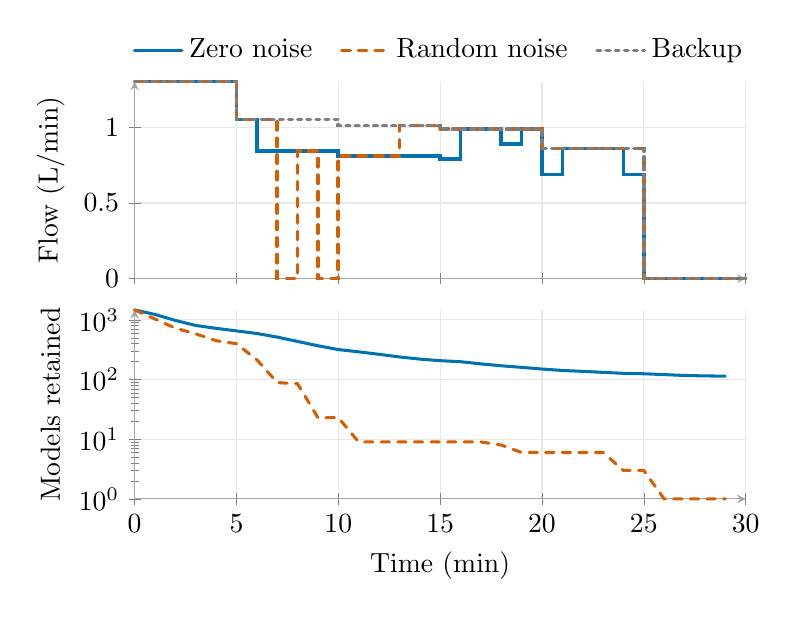
\begin{tikzpicture}
\begin{axis}[width=0.64\linewidth,
 height=2.5cm,
 scale only axis,
 xlabel={},
 ylabel={Flow (L/min)},
 axis lines=left,
 axis line style={gray!70},
 grid=major,
 grid style={gray!18},
 tick label style={font=\normalsize},
 label style={font=\normalsize},
 every axis plot/.append style={line cap=round},
 clip=false,
 xmin=0,
 xmax=30,
 ymin=0,
 legend style={font=\normalsize,draw=none,fill=none,at={(0.5,1.04)},anchor=south,/tikz/every even column/.append style={column sep=8pt},legend columns=3,},
 name=feedbacktop,xticklabels={}]
\addplot[color=main,line width=1.3pt,no marks] coordinates {(0,1.30366) (1,1.30366) (1,1.30366) (2,1.30366) (2,1.30366) (3,1.30366) (3,1.30366) (4,1.30366) (4,1.30366) (5,1.30366) (5,1.05375) (6,1.05375) (6,0.843002) (7,0.843002) (7,0.843002) (8,0.843002) (8,0.843002) (9,0.843002) (9,0.843002) (10,0.843002) (10,0.809357) (11,0.809357) (11,0.809357) (12,0.809357) (12,0.809357) (13,0.809357) (13,0.809357) (14,0.809357) (14,0.809357) (15,0.809357) (15,0.790698) (16,0.790698) (16,0.988372) (17,0.988372) (17,0.988372) (18,0.988372) (18,0.889535) (19,0.889535) (19,0.988372) (20,0.988372) (20,0.688111) (21,0.688111) (21,0.860138) (22,0.860138) (22,0.860138) (23,0.860138) (23,0.860138) (24,0.860138) (24,0.688111) (25,0.688111) (25,0) (26,0) (26,0) (27,0) (27,0) (28,0) (28,0) (29,0) (29,0) (30,0)};\addlegendentry{Zero noise}
\addplot[color=accent,line width=1.3pt,no marks,dashed] coordinates {(0,1.30366) (1,1.30366) (1,1.30366) (2,1.30366) (2,1.30366) (3,1.30366) (3,1.30366) (4,1.30366) (4,1.30366) (5,1.30366) (5,1.05375) (6,1.05375) (6,1.05375) (7,1.05375) (7,0) (8,0) (8,0.843002) (9,0.843002) (9,0) (10,0) (10,0.809357) (11,0.809357) (11,0.809357) (12,0.809357) (12,0.809357) (13,0.809357) (13,1.0117) (14,1.0117) (14,1.0117) (15,1.0117) (15,0.988372) (16,0.988372) (16,0.988372) (17,0.988372) (17,0.988372) (18,0.988372) (18,0.988372) (19,0.988372) (19,0.988372) (20,0.988372) (20,0.860138) (21,0.860138) (21,0.860138) (22,0.860138) (22,0.860138) (23,0.860138) (23,0.860138) (24,0.860138) (24,0.860138) (25,0.860138) (25,0) (26,0) (26,0) (27,0) (27,0) (28,0) (28,0) (29,0) (29,0) (30,0)};\addlegendentry{Random noise}
\addplot[color=muted,line width=1.3pt,no marks,dotted] coordinates {(0,1.30366) (1,1.30366) (1,1.30366) (2,1.30366) (2,1.30366) (3,1.30366) (3,1.30366) (4,1.30366) (4,1.30366) (5,1.30366) (5,1.05375) (6,1.05375) (6,1.05375) (7,1.05375) (7,1.05375) (8,1.05375) (8,1.05375) (9,1.05375) (9,1.05375) (10,1.05375) (10,1.0117) (11,1.0117) (11,1.0117) (12,1.0117) (12,1.0117) (13,1.0117) (13,1.0117) (14,1.0117) (14,1.0117) (15,1.0117) (15,0.988372) (16,0.988372) (16,0.988372) (17,0.988372) (17,0.988372) (18,0.988372) (18,0.988372) (19,0.988372) (19,0.988372) (20,0.988372) (20,0.860138) (21,0.860138) (21,0.860138) (22,0.860138) (22,0.860138) (23,0.860138) (23,0.860138) (24,0.860138) (24,0.860138) (25,0.860138) (25,1.35003e-13) (26,1.35003e-13) (26,1.35003e-13) (27,1.35003e-13) (27,1.35003e-13) (28,1.35003e-13) (28,1.35003e-13) (29,1.35003e-13) (29,1.35003e-13) (30,1.35003e-13)};\addlegendentry{Backup}
\end{axis}
\begin{axis}[width=0.64\linewidth,
 height=2.4cm,
 scale only axis,
 xlabel={Time (min)},
 ylabel={Models retained},
 axis lines=left,
 axis line style={gray!70},
 grid=major,
 grid style={gray!18},
 tick label style={font=\normalsize},
 label style={font=\normalsize},
 every axis plot/.append style={line cap=round},
 clip=false,
 xmin=0,
 xmax=30,
 ymin=1,
 ymode=log,at={(feedbacktop.south)},anchor=north,yshift=-0.4cm]
\addplot[color=main,line width=1.1pt,no marks,forget plot] coordinates {(0,1465) (1,1231) (2,978) (3,805) (4,721) (5,653) (6,591) (7,514) (8,435) (9,368) (10,318) (11,291) (12,265) (13,239) (14,220) (15,207) (16,199) (17,183) (18,170) (19,160) (20,150) (21,142) (22,137) (23,132) (24,127) (25,125) (26,121) (27,117) (28,115) (29,114)};
\addplot[color=accent,line width=1.1pt,dashed,no marks,forget plot] coordinates {(0,1465) (1,1032) (2,727) (3,582) (4,448) (5,398) (6,215) (7,89) (8,85) (9,23) (10,23) (11,9) (12,9) (13,9) (14,9) (15,9) (16,9) (17,9) (18,8) (19,6) (20,6) (21,6) (22,6) (23,6) (24,3) (25,3) (26,1) (27,1) (28,1) (29,1)};
\end{axis}
\end{tikzpicture}
\caption{Observation-dependent replenishment}\label{fig:feedback}
\end{figure}
A separate matched 12-model ablation uses 26.00 L without observations versus 22.86, 22.86 and 22.08 L with them in three structures. Six feedback trajectories pass 18 independent half-second three-grid RHS/energy replays; realized actions do not certify fine-grid feedback throughout the bank.

Minute-10 shifts to 45°C supply or 40 W/(m² K) surface loss empty the set at minute 11; terminal bias intervals independently exclude all 23 preceding survivors. Neither partial service counts as savings. An empty set invalidates reuse, without identifying the cause or certifying recovery.

\subsection{Parameter changes and fixed-policy bounds}
Six predeclared bank-external truths give two complete services (22.59/22.80 L commands). Changed storage, dimensions, supply or loss empties the bank after 28/5/11/9 minutes, before a checked temperature violation. Partial services are not savings; Section 12 separately tests limited recourse.

Fix those commands, baseline geometry, uniform 40°C initial water, 34°C contact, 50°C inlet and 22°C air. Static $(D,h_s,h_b,\alpha)$ center is $(0.001025,24.375,26.25,1.0125)$; halfwidths $6.25\times10^{-06}$ m²/s, 0.15625/0.3125 W/(m² K), 0.003125. These mathematical neighborhoods are not measured tolerances.

\textbf{Fixed-command perturbation bound.} Write $U^{\prime}=M_\theta U+c_\theta$, affine in the four parameters. For halfwidths $w_j$, set $K_j=w_j\partial_jM$, $f_j=w_j\partial_jc$, and $\theta=\theta_0+w\odot z$ with $|z_j|\le1$. Nominal variations satisfy $S_j^{\prime}=M_0S_j+K_jU_0+f_j$, $S_j(0)=0$.

\begin{proof}
The exact remainder $r=U_\theta-U_0-\sum_jz_jS_j$ satisfies

\begin{equation}r^{\prime}=M_\theta r+\sum_{j,k}z_jz_kK_jS_k,\qquad r(0)=0.\end{equation}
Positive parameters give nonnegative off-diagonals and nonpositive row sums at every vertex, hence throughout the affine box. Contraction [10] and variation of constants give

\begin{equation}\|r(t)\|_\infty\le R(t),\qquad R(t)=\sum_{j,k}\int_0^t\|K_jS_k(u)\|_\infty\,du.\end{equation}
The cellwise radius is $\sum_j|S_j|+R$: subtract it for the floor, add it for the ceiling, and twice for spread. States are continuous at flow switches; $R$ accumulates across them.

\end{proof}
Half-second derivative/chord bounds assume $2\times10^{-6}$°C, $2\times10^{-6}$°C/s and $2\times10^{-6}$°C/s² errors. Of halfwidth scales 4/2/1/0.4, the displayed box is the largest passing both fixed paths on all three meshes: floor $\geq$39.0759°C, ceiling $\leq$40.7769°C, spread $\leq$1.1746°C; extra planning reserves do not all pass. Independent RHS/energy checks cover 102 corners/centers, not the continuum. A prior defect bound certified none. This exact-remainder box assumes numerical accuracy and covers fixed commands, not all feedback branches or real baths.

\subsection{Transport comparison and network infeasibility}
A separate axial closure matches volume, storage and total conductances, with uniform/localized-body losses but different anatomy. With v=qL/V, loss per length $\lambda$ and capacity per length c,

\begin{equation}T_t=D T_{xx}-vT_x-\lambda(x,T)/c,\qquad vT(0)-DT_x(0)=vT_{\mathrm in},\quad T_x(L)=0.\end{equation}
The flux inlet [11] conserves enthalpy. Both policies replay two loss profiles on 40/80/160 meshes at $D$=0.0003/0.001/0.003 m²/s. Under constant flow, weak-mixing mean/outlet ends at 39.444/38.581°C. N80 searches choose start 0 min at $D$=0.001 (22.71/22.68 L, uniform/local loss), or 10 min at $D$=0.003 (18.87/18.86 L); all selected candidates pass three-mesh sampled checks.

Starts 0:120:1200 s and first roots 0:0.2:3 L/min use floor 39.03°C. Neither weak-mixing profile accepts a root; this finite search is inconclusive.

\textbf{An arbitrary-control obstruction.} Fix $D=0.0003$ m²/s, 34°C contact, 40°C initial water, the original route and 30 minutes. No measurable $q(t)\in[0,3]$ L/min satisfies the 39°C all-cell floor, 41°C ceiling outside the inlet jet zone and 1.5°C spread on the 96-cell network.

Let $\theta=T-39\in P$, with P enforcing the floor, ceiling, jet barrier and spread. Write $\theta^{\prime}=K\theta+b+q(S\theta+a)$. For signed $\omega$, define $E=\omega^T\theta$, $E_{\min}=\min_P E$ and $R=\max_{q\in\{0,3\},\theta\in P}\omega^T\theta^{\prime}$. Then

\begin{equation}E_{\min}\le E(t)\le E(0)+tR,\qquad t\le\frac{E(0)-E_{\min}}{-R}\quad(R<0).\end{equation}
The derivative is affine in the common $q$: endpoints bound every measurable policy, and integration gives the inequality. Frozen weights contrast inlet-near warmth with the remote end; E is not heat. Exact rational support bounds give safety time <1717 s. Timing alone cannot reach 1800 s. The tested stronger-diffusion cases lose this obstruction, without proving feasibility.

Frozen-dual box corrections give a concave piecewise-affine gap $g=E_{\min}^{\rm lower}-E(0)-1800R_{\rm upper}$: $s=D/0.0003$, $\ell$ scales both losses, z limits spread. Positive g certifies convex exclusion. Exact roots give 0.00029047 < $D$ < 0.00030957 m²/s at original loss and 1.5°C spread. At $D$=0.0003, separately, loss scales 0.97894–1.2 or spreads 0.75–1.53242°C remain excluded with other inputs fixed. These inward-rounded boundaries do not establish feasibility. Original 288-cell relaxations remain inconclusive.

A fixed 0.15 m ball at $(0,W/2,H)$ gives residual bounds >0.115/0.217/0.179°C on 96/288/768 cells; time limits <1619/<1481/<1533 s. Only the mask changes: non-nested on 96, stricter on 288. The source lane still follows the grid. These are finite-network obstructions, not a continuum limit or a verdict for the original 288-cell target.

\begin{equation}E_{\mathrm excess}=\rho c_p\int q(T_{\mathrm out}-\overline T)\,dt.\end{equation}
Positive excess is extra overflow loss relative to the mean. Original/matched-axial values are $-31.51/-26.28$ kJ. Both outlets are cooler: a permitted short circuit does not establish the cause of the water penalty.

For uniform loss, $k=(H_a+H_b)/C$, $w=T_x$ obeys $w_t=Dw_{xx}-vw_x-kw$, $w(L)=0$, $w(0)=v[T(0)-T_{\rm in}]/D\le0$ when $T\le T_{\rm in}$. Uniform initial water and inherited gradients at switches permit the maximum principle: $w\le0$, hence $T_{\rm out}\le\overline T$. Localized loss adds gradient forcing.

Steady/Robin tests show first-order convergence (N160 error $\leq$0.002614°C); six independent flux/RK45 differences $\leq$$3.30\times10^{-07}$°C and energy errors $\leq$0.00213 J verify this closure, not real baths or PDE-wide feasibility.

\FloatBarrier
\section{Decision synthesis and recourse}
The strategy follows the thermal bottleneck. The 24.14 L constant trickle starts at minute zero: its 1°C allowance is a temperature constraint, not a trigger to begin heating. The separately qualified 21.48 L schedule waits five minutes, supplies for fifteen and coasts for ten, saving 11\%. Heat must start travelling before a distant cold region reaches its limit. Under uncertain loss, delivery and contact structure, the 26.09 L common-reserve backup supplies a continuation for the finite compatible bank; its observation-dependent reductions are conditional, not universal schedules.

Geometry and body contact alter both storage and heat paths. Faster modeled mixing can support waiting, while surface loss offsets its saving and foam reduces that loss. A mean or two equal readings cannot certify uniformity: a changed geometry or motion needs a newly checked continuation.

Over the remaining horizon, for every compatible model: \textbf{wait} only with a qualified zero-flow bridge and backup; \textbf{replenish} with a checked continuation or backup; otherwise \textbf{reassess}.

\begin{samepage}
\indent Reconstruct 54 exposed static hypotheses from 40°C/34°C and all actions/readings: six structures × $D$ factors 0.975/1/1.025 × surface-loss offsets -0.625/0/0.625 W/(m² K). Intersect shared-bias intervals without using truth states. With prior parallel maintenance, pre-reading sets 1/15/6/7 qualify a 60 s bridge; the last reading leaves 1/8/4/6. Tail search: 0:0.05:2 L/min (Table \ref{tab:recourse}).
\par
\end{samepage}

\begin{table}[ht]\centering\normalsize\caption{Recourse after a one-minute bridge}\label{tab:recourse}
\begin{tabular}{@{}>{\raggedright\arraybackslash}p{0.3333\dimexpr\linewidth-6\tabcolsep\relax}>{\raggedright\arraybackslash}p{0.1880\dimexpr\linewidth-6\tabcolsep\relax}>{\raggedright\arraybackslash}p{0.2222\dimexpr\linewidth-6\tabcolsep\relax}>{\raggedright\arraybackslash}p{0.2564\dimexpr\linewidth-6\tabcolsep\relax}@{}}
\toprule
Changed condition & Alarm (min) & Tail (L/min) & Total command (L) \\ \midrule
Contact storage & 28 & 0.00 & 22.17 \\
Longer geometry & 5 & 0.80 & 25.72 \\
Cooler inlet & 11 & 0.80 & 25.86 \\
Higher loss & 9 & 1.05 & 30.76 \\ \bottomrule
\end{tabular}
\end{table}
Chord bounds cover bridge/tail; 57 independent three-grid sampled paths cover 19 survivors at physical 39/41/1.5°C limits without old reserves. Prior 0.70 L/min fails all meshes; higher-loss completion exceeds 26.09 L. Empty sets, failed bridges or timeouts refuse action in this offline study.

A predeclared off-bank case ($D$=0.00101225 m²/s, surface coefficient 31.50 W/(m² K)) retains a nine-minute prefix without a new alarm. Five of seven bridge hypotheses survive; a 1.05 L/min tail commands 30.76 L and delivers 31.14 L. Eighteen sampled three-grid paths include the truth, which never initializes decisions.

\clearpage
\section{Practical guidance}
\subsection*{A guide for the person in the bathtub}
\textbf{Choose a temperature range, then choose the timing.} Our example starts with 164 L at 40°C and lasts 30 minutes. Allowing the water to be as much as 1°C cooler needs 24.14 L with a constant trickle of about 0.805 L/min from minute zero. The 1°C allowance is not an instruction to wait until the bath has cooled by 1°C. With a 2°C allowance, the modeled constant trickle needs about 1.9 L. These are different service choices for the example tub.

\textbf{Send warmth to the cold end in time.} Water near the faucet can stay warm while a distant corner cools. Heat takes time to reach that corner, so turning on the water only when it reaches your lower limit can be too late. Gentle movement can redistribute heat, but stronger motion may increase surface loss: our stronger-mixing example needs 19.40 L, rising to 23.04 L with greater surface loss. Two equal thermometer readings do not show that the whole bath is even.

\textbf{A different, calibrated schedule can save water.} The separately checked nominal example keeps the faucet off from minutes 0–5; supplies about 1.67, 1.34 and 1.28 L/min in minutes 5–10, 10–15 and 15–20 respectively; then stops for minutes 20–30. It uses 21.48 L in the calculation, against 24.14 L for the immediate constant trickle. Those rates are rounded illustrations; Section 7.1 gives the exact calculated settings. Accurate flow control and temperature checks are needed: only 74\% of the specified random tap-error trials stayed within the limits. A poorly mixing bath may need earlier heating rather than a larger late burst.

\textbf{Measure and calibrate before relying on automatic adjustments.} The modeled controller checks two temperatures every minute and adjusts flow using a bath-specific cooling and heat-distribution model prepared in advance. It reduces or stops flow only while that model still supports the chosen temperature range for the rest of the bath; otherwise it keeps its prechecked backup settings. Unexplained readings require reassessing the supply, movement and heat loss. Two probes alone cannot rule out a cold corner that the model missed. Four specified modeled changes allowed replacement plans after a checked one-minute pause, sometimes with more water; unchecked changes have no such assurance.

\textbf{Account for the tub and the person.} At the same volume, a deep, narrow tub exposes less top surface: our example needs 17.48 L rather than 24.14 L. Greater displacement and contact area raise demand to 28.11 L. Body shape changes where heat is removed, and warmer skin reduces heat uptake. A larger fill can need less replacement but more initial water, so count both. An intact bubble layer may slow surface cooling; our assumed layer lowers replacement to 10.37 L. Its effect depends on the additive and whether movement breaks the layer.

\textbf{Count preparation too.} Across the broader model bank, cooling-only and hot-water trials lead to fixed schedules using 26.09/23.63 L per bath. One reusable 6 L hot-water trial pays back from use 3 only when conditions and reset costs match. Each trial takes 30 minutes and each service starts uniformly at 40°C. These trial costs differ from the automatic-controller comparison. Keep the hot jet away from skin: the model tracks water-cell averages and does not certify jet or skin-film temperature.

\clearpage
\section{References and reproducible algorithm}
\begingroup\normalsize\setlength{\parindent}{0pt}\hangindent=1.5em [1] COMAP. 2016 MCM Problem A: A Hot Bath. 2016. Official problem PDF: \url{https://contest.comap.com/undergraduate/contests/mcm/contests/2016/problems/2016_MCM_Problem_A.pdf}.\par\endgroup
\begingroup\normalsize\setlength{\parindent}{0pt}\hangindent=1.5em [2] U.S. Department of Energy. DOE Fundamentals Handbook: Thermodynamics, Heat Transfer, and Fluid Flow. DOE-HDBK-1012/2-92, June 1992. Convection heat transfer, Eq. (2-9).\par\endgroup
\begingroup\normalsize\setlength{\parindent}{0pt}\hangindent=1.5em [3] IAPWS. Revised Release on the IAPWS Formulation 1995 for the Thermodynamic Properties of Ordinary Water Substance for General and Scientific Use. R6-95(2018). \url{https://iapws.org/technical-guidance/release/IAPWS-95}.\par\endgroup
\begingroup\normalsize\setlength{\parindent}{0pt}\hangindent=1.5em [4] SciPy developers. scipy.sparse.linalg.expm\_multiply and scipy.integrate.solve\_ivp, API documentation. \url{https://docs.scipy.org/doc/scipy/reference/}. Accessed 7 October 2026.\par\endgroup
\begingroup\normalsize\setlength{\parindent}{0pt}\hangindent=1.5em [5] Bergman, T. L., Lavine, A. S., Incropera, F. P., DeWitt, D. P. Fundamentals of Heat and Mass Transfer, 7th ed. Wiley, 2011. Natural convection above a heated horizontal surface (characteristic length A/P); heat and mass transfer analogy.\par\endgroup
\begingroup\normalsize\setlength{\parindent}{0pt}\hangindent=1.5em [6] Menzies, C., Clarke, N., Steward, C. J., Thake, C. D., Pugh, C. J. A., Cullen, T. Vascular, inflammatory and perceptual responses to hot water immersion: impacts of water depth and temperature in young healthy adults. Experimental Physiology, 2025. doi:10.1113/EP092761.\par\endgroup
\begingroup\normalsize\setlength{\parindent}{0pt}\hangindent=1.5em [7] OpenAI, Codex (GPT-6-based assistant), and Anthropic, Claude Sonnet 5.5 in Claude Code. Used during 7–10 October 2026 for modeling, code, validation and report composition; exact builds not independently established. See Report on Use of AI.\par\endgroup
\begingroup\normalsize\setlength{\parindent}{0pt}\hangindent=1.5em [8] Munk, W. H., Anderson, E. R. Notes on a theory of the thermocline. Journal of Marine Research, 7(3), 276–295, 1948.\par\endgroup
\begingroup\normalsize\setlength{\parindent}{0pt}\hangindent=1.5em [9] NASA/NPARC Alliance. Verification Assessment and Validation Assessment, CFD tutorial. \url{https://www.grc.nasa.gov/WWW/wind/valid/tutorial/}. Accessed 9 October 2026.\par\endgroup
\begingroup\normalsize\setlength{\parindent}{0pt}\hangindent=1.5em [10] Higham, N. J. What Is the Logarithmic Norm? 18 January 2022. \url{https://nhigham.com/2022/01/18/what-is-the-logarithmic-norm/}. Theorems 3 and 6. Accessed 10 October 2026.\par\endgroup
\begingroup\normalsize\setlength{\parindent}{0pt}\hangindent=1.5em [11] COMSOL. Theory for the Inflow Boundary Condition. Heat Transfer Module documentation, version 6.3. \url{https://doc.comsol.com/6.3/doc/com.comsol.help.heat/heat_ug_theory.07.009.html}. Accessed 10 October 2026.\par\endgroup
\subsection*{Reproduction and computational record}
The inherited baseline network, exact flow settings and independent numerical checks are available through the public Praxis MCM-2016-A reproduction index: \url{https://github.com/WJSGZZ/praxis/tree/0e3f29b1323486eafa74916218e72cfcb066631a/demos/mcm-2016-a/reproduce}. Its reference/results.json gives baseline inputs; reference/mesh\_check.json binds the six-stage rates and continuous checks; reference/whole-horizon-exclusion.md locates the exact control certificate. The present private learning increment is separately indexed at outputs/praxis-three-strong-o-20261013/authors/MCM-2016-A/reproduction-index.md in its supplied workspace: it links cases/strong-o-2016-a/code/model.py, code/validate.py and run 20261013T015532-1eed61b2 to the new mixing diagnostic. This new increment has not been published.

AI assistance in the inherited calculations and this learning revision is attributed to [7]; the separate Report on Use of AI records author, coordinating-agent and author-external checks. The published mathematics and numerical error assumptions, rather than an AI judgment, determine the stated evidence scope.

Assemble valid capacities, symmetric exchange and conservative inlet/overflow; compute mixed benchmarks; search floor crossings, reject ceiling/spread failures and rank water costs. Qualify buffered schedules on three meshes; repeat searches at Sobol draws. Independent RHS/RK45 uses rtol $2\times10^{-9}$, atol $2\times10^{-10}$°C, steps $\leq$5 s and energy/analytic checks. Axial tests and AI use: Section 11.4 and [7].

\section*{Appendix A. Scenario definitions}
\addcontentsline{toc}{section}{Appendix A. Scenario definitions}
Each row in Table \ref{tab:12} changes only the listed baseline inputs. All unspecified inputs remain as stated in Section 2; geometry and conductance are then rebuilt. The equal-volume aspect-ratio cases retain the envelope volume of 0.22425 m³. Widths s describe a smooth displacement distribution, not measured anatomical semiaxes.

Accepted candidates are independently replayed on their scenario network at intervals of no more than five seconds. These scenario checks are sampled checks; continuous-time envelopes are reported for the baseline constant rate and the selected scheduled policy; the latter uses additional interval refinement when necessary. “None accepted” refers to the documented finite search and is not an infeasibility theorem.

\begin{table}[ht]\centering\normalsize\caption{Scenario definitions}\label{tab:12}
\begin{tabular}{@{}>{\raggedright\arraybackslash}p{0.3077\dimexpr\linewidth-2\tabcolsep\relax}>{\raggedright\arraybackslash}p{0.6923\dimexpr\linewidth-2\tabcolsep\relax}@{}}
\toprule
Scenario & Changed input(s) \\ \midrule
Weak Mixing & $D$ (m²/s) = 0.0003 \\
Strong Mixing & $D$ (m²/s) = 0.003 \\
Moving With Added Surface Loss & $D$ (m²/s) = 0.003; surface coefficient (W/m²K) = 30 \\
Loose Comfort & lower limit (°C) = 38 \\
Tight Comfort & lower limit (°C) = 39.5 \\
Foam & surface multiplier = 0.4 \\
Shallow Wide & length (m) = 1.7; width (m) = 0.75; depth (m) = 0.175882 \\
Deep Narrow & length (m) = 1.3; width (m) = 0.6; depth (m) = 0.2875 \\
Small Bath & depth (m) = 0.2 \\
Large Bath & depth (m) = 0.27 \\
Deep Bath & depth (m) = 0.35 \\
Larger Body & body displacement (m³) = 0.075; body contact area (m²) = 1.35 \\
Long Body & body widths s (m) = [0.48, 0.12, 0.1] \\
Warmer Skin & skin temperature (°C) = 36 \\
Cooler Skin & skin temperature (°C) = 32 \\
High Loss & surface coefficient (W/m²K) = 36; wall coefficient (W/m²K) = 8.5; body coefficient (W/m²K) = 40 \\
Low Loss & surface coefficient (W/m²K) = 17; wall coefficient (W/m²K) = 4.5; body coefficient (W/m²K) = 12 \\
Stratified & vertical/horizontal $D$ ratio = 0.2 \\
Convective Surface Layer & vertical/horizontal $D$ ratio = 3 \\
Cool Supply & inlet temperature (°C) = 45 \\ \bottomrule
\end{tabular}
\end{table}
\clearpage
\section*{Report on Use of AI}
\addcontentsline{toc}{section}{Report on Use of AI}
\subsection*{Tools and tasks}
Codex (GPT-6-based) and Claude Sonnet 5.5 via Claude Code assisted the earlier modeling, calculations, checks, figures and writing during 7–10 October 2026; exact builds are unverified. The 13 October learning revision used a Codex author sub-agent to read the original task/current 26-page seed, reorganize the argument and add a mathematical mixing diagnostic. An author-external Codex reviewer reconstructed the principal strategies, mixing spectrum, delay bounds and a guide-trigger counterexample; the coordinating Codex agent independently checked the mixing operator and confirmed the action correction. The author revised the source and reader guide in response. No real bath experiment, live control or human correctness check was performed.

\subsection*{Material exposure}
The earlier post-seal learning used same-task papers 44845/54164 and COMAP commentary. That exposure is preserved; this revision is not unseen-problem testing. The current author read own source, raw task and retained scientific archives; no new student answer or Outstanding original was read. Official 2016 problem-index metadata was checked for delivery boundaries. Other task registration metadata were visible, without their papers or scientific arrays.

\subsection*{Outputs and verification}
The previous 21.48 L control, continuous mesh checks, observation-compatible banks, structural alternatives, parameter boxes, feedback, rejection/recourse and finite-network certificates were retained with their original byte identities. Historical failed candidates, inconclusive finer relaxations and timeouts remain. The new diagnostic diagonalizes the symmetric closed-exchange network; an independent edge assembly, direct pair-flux integration, conservation balance and all 96 analytic empty-grid cosine eigenvalues check its mathematics. It also constructs a two-mode probe counterexample and enumerates the existing bank diffusivity projections. No baseline optimization or expensive historical study was restarted.

\subsection*{Sources and limits}
The inherited record states direct reading of [1]–[4]/[6]/[10]–[11], with the [5]/[8] coefficient relations checked indirectly. These references support the same scope as in the seed; later publication dates make this a present-day study of the 2016 task. The numerical mixing diagnostic isolates a mathematical closure, not measured human motion. The new source, arrays, independent checks, original receipts, full-PDF review and separate first-complete/final seals are retained privately. Task/tool records are available; a complete transcript and exact model usage are unavailable.


\end{document}
